\documentclass{article}
\usepackage[utf8]{inputenc}
\usepackage[T1]{fontenc}
\usepackage{lmodern}
\usepackage{authblk}
\usepackage{setspace}
\usepackage{etoolbox}
\usepackage[margin=1in]{geometry}
\usepackage{graphicx}
\graphicspath{ {./figures/}{../arxiv/figures/} }
\usepackage{subcaption}
\usepackage{amsmath}
\usepackage{amssymb}
\usepackage{amsthm}
\usepackage{url}
\usepackage{float}
\usepackage[section]{placeins}
\usepackage[font=small,labelfont=bf,labelsep=period]{caption}
\usepackage{longtable,booktabs,array,calc,tabularx}

%%%%%% Bibliography %%%%%%
\usepackage[style=nejm,
citestyle=numeric-comp,
sorting=none,
backend=bibtex]{biblatex}
\addbibresource{references.bib}

\usepackage[hidelinks]{hyperref}

\theoremstyle{plain}
\newtheorem{proposition}{Proposition}
\theoremstyle{remark}
\newtheorem*{remark}{Remark}

%%%%%% Title %%%%%%
\title{Input Constraints and Learning Dynamics in Predictive World Models}

\author[1*]{Somesh Mohapatra}
\affil[1]{Independent.}
\affil[*]{Address correspondence to: pikulsomesh@gmail.com}
\date{}

\setstretch{1.2}
\setlength{\parskip}{0.3em}
\sloppy
\AtBeginEnvironment{longtable}{\small}

\begin{document}

\maketitle

\begin{abstract}
Predictive world models are usually trained on clean, shuffled data at full quality from the first update. We study how learning changes when the training stream is instead degraded, staged over time and split across modalities. We model each constraint as a fixed degradation operator applied to one modality and derive four short results: an information bound on what any representation of filtered input can retain; an exact learning-time law for a linear read-out under gradient flow, in which scaling input contrast by a factor \(\kappa\) delays learning by a factor \(\kappa^{-2}\) while Gaussian blur mainly lowers the reachable ceiling; a plateau after function-preserving widening, because new units receive gradient only through their zero-initialised outgoing weights; and a conditional-mean account showing that a squared-error forecaster is more surprised by an occluded object's reappearance than by its disappearance when reappearance is uncertain. We test each result on small Adam-trained networks in a synthetic multisensory environment, with one predictive world model per modality (convolutional encoder, residual latent dynamics, spatial-broadcast decoder) and a fusion model trained with random modality masking, across six training curricula and two front-end ablations, 5 seeds each. The most degraded stage slows the linear solution 39-fold, and the trained vision model reaches position \(R^2\) 0.02 where a supervised network on the same input reaches 0.60; the ablations attribute this lag to contrast, not blur. A degraded-to-clean curriculum costs vision a little and helps audio localisation, mainly as augmentation; network growth halves parameter-updates but slows learning; and fusion tracks an occluded object better than any single modality. All results are from a small synthetic setting; transfer to larger models and real data is untested.
\end{abstract}

\section{Introduction}
\label{sec:intro}

Predictive world models learn a compact internal model of an environment and use it to forecast what follows from what they observe and do \autocite{ha2018world}. LeCun argues that such models, learned by prediction in an abstract representation space rather than in pixels, are a missing ingredient of autonomous intelligence \autocite{lecun2022path}, and joint-embedding predictive architectures (JEPA) put the idea into practice for images and video \autocite{assran2023self,bardes2024revisiting,garrido2025intuitive}. Li describes world models as generative, multimodal and interactive systems that predict the next state of a scene given an action \autocite{li2025words}. These systems are trained on very large corpora, yet training datasets are projected to reach roughly the size of the stock of public human-written text between 2026 and 2032 \autocite{villalobos2024will}, and multisensory, embodied data are scarcer still. How a training stream is degraded, staged and ordered may therefore matter as well as how large it is.

Curriculum learning orders training data from easy to hard \autocite{bengio2009curriculum}, and the evidence for it is mixed. Starting with blurred or colourless images can make recognition more robust \autocite{vogelsang2018potential,vogelsang2024impact}, slowly changing video helps self-supervised learning \autocite{sheybani2023curriculum}, and deep networks show critical periods, including for multisensory integration \autocite{achille2019critical,kleinman2023critical}. Yet the benefit of ``starting small'' \autocite{elman1993learning} was challenged by later simulations \autocite{rohde1999language}, ordered training helps little on standard benchmarks and mostly when training time is short or labels are noisy \autocite{wu2021curricula}, and stage-like learning can arise from gradient dynamics alone \autocite{saxe2019mathematical}. What is missing is an account of \emph{how} a given input constraint changes the dynamics of learning, specific enough to predict which constraint matters and by how much.

We study this question for predictive world models trained to forecast their own input. We model each constraint as a fixed, non-learned degradation operator \(\Phi_s(\cdot;a)\) applied to modality \(s\) at curriculum stage \(a\), and we consider three levers: input quality (contrast, blur, colour, noise), the order in which quality changes, and network capacity, which can grow by function-preserving widening \autocite{chen2016net2net}. We derive four short propositions about this setting. Proposition~\ref{prop:info} bounds what any representation of the filtered input can retain. Proposition~\ref{prop:time} gives the exact learning trajectory of a linear read-out under gradient flow and shows that contrast sets its speed while blur sets its ceiling. Proposition~\ref{prop:growth} shows that widened units start to learn only through their outgoing weights, which predicts a plateau after each widening. Proposition~\ref{prop:surprise} shows that the conditional-mean forecast of a squared-error model is more surprised by an occluded object's reappearance than by its disappearance whenever reappearance has probability below one half. The tools are standard (the data-processing inequality, the eigen-decomposition of linear gradient flow, and the bias--variance decomposition); the contribution is to apply them to staged, degraded, multimodal training and to test each prediction in trained nonlinear networks.

The experiments use a small synthetic environment rendered into four streams (\(32\times32\) colour vision, binaural spectra, an \(8\times8\) tactile patch and proprioception), with one predictive world model per modality and a fusion model over their frozen latents trained with random modality masking \autocite{neverova2016moddrop}. Six training curricula cross the input schedule (clean throughout, degraded-to-clean, shuffled quality, clean-to-degraded) with capacity (fixed or grown), and two ablations isolate contrast and blur. All networks are trained with Adam \autocite{kingma2015adam}, for which the theory is not exact, so the experiments test how far the linear predictions carry over. Whether the effects hold with larger networks, richer scenes and real video is not tested here.

\textbf{Motivation from biological learners.} The degradation operators are parameterised from measurements of human sensory development. Newborn visual acuity is roughly one thirtieth of the adult value and contrast sensitivity a small fraction of it \autocite{banks1988optical,norcia1985spatial}; touch and hearing function earlier than vision, and the order in which senses come online may shape how they are combined \autocite{turkewitz1982limitations}. Children nevertheless learn from a few thousand waking hours of such input \autocite{smith2018curriculum}, and networks trained on one child's head-camera video learn useful visual representations and word meanings \autocite{orhan2020self,orhan2024learning,vong2024grounded}. We use these schedules only as a realistic, pre-specified curriculum to ablate against. Each curriculum stage is indexed by \(a\in\{0,3,6,12\}\), the age in months whose published sensory parameters set the operator; \(a\) indexes input quality only, and no part of any network is switched on or off by it.

\textbf{Companion paper.} The same environment and degradation operators underlie a companion manuscript on sensory perception \autocite{mohapatra2026senses}. Shared with it: the operator parameter tables (Table~\ref{tab:frontends} here), the information-ceiling and own-stage probe data for vision and hearing (Fig.~\ref{fig:development} and Extended Data Fig.~S3 here, plotted differently there), and the finding that the ceiling-based half-stage measure does not recover the biological order of maturation (Appendix~\ref{app:milestones}). New in this paper: the formal problem, the four propositions and proofs, the spectral analysis, the six curricula with statistics and the ablations, the growth analysis, the fusion model, the violation-of-expectation analysis and the follow-up experiments of Extended Data Fig.~S4. The latent-prediction vision model is the same in both papers; its surprise at the disappearance events is reported only here.

\section{Problem setting and model}
\label{sec:model}

\subsection{Staged, degraded, multimodal input}

A scene state \(s_t\) evolves under an action \(u_t\in\mathbb R^2\). Each modality \(s\) delivers a clean observation \(o_t^{s}\), a deterministic function of the scene, and a property \(Y_t=g(s_t)\), such as the position or identity of an object, is the quantity we ask a representation to retain. At curriculum stage \(a\) the learner instead receives
\begin{equation}
\tilde o_t^{s}=\Phi_s(o_t^{s};a),
\label{eq:frontend}
\end{equation}
where \(\Phi_s\) is a fixed degradation operator (``front end'') whose parameters are interpolated in \(a\) from Table~\ref{tab:frontends}. For vision, with acuity \(\mathrm{cpd}(a)\) in cycles per degree, contrast sensitivity \(\mathrm{CS}(a)\) and colour saturation \(\gamma(a)\), the operator blurs, compresses contrast towards the image mean and desaturates:
\begin{equation}\sigma(a)=\tfrac12\cdot\frac{30}{\mathrm{cpd}(a)}\cdot\frac{32}{224},\qquad x=G_{\sigma(a)}*o,\qquad x\leftarrow \bar x+\kappa(a)\,(x-\bar x),\qquad \kappa(a)=\mathrm{clip}\!\left(\tfrac12\log_{10}\mathrm{CS}(a),\,0.15,\,1\right),\label{eq:vision}\end{equation}
\begin{equation}\tilde o=\mathrm{clip}_{[0,1]}\big(\ell+\gamma(a)(x-\ell)\big),\qquad \ell=0.299x_R+0.587x_G+0.114x_B,\end{equation}
where \(G_\sigma\) is a separable Gaussian with replicate padding and \(\bar x\) the image mean. The contrast factor \(\kappa(a)\) and the blur width \(\sigma(a)\) are the two quantities the theory separates. The log compression replaces a linear gain \(\mathrm{CS}/100\), which would leave 2\% of contrast at \(a=0\); contrast sensitivity is a threshold, not a gain. The audio operator blurs along frequency, attenuates high frequencies, shrinks the interaural difference and adds noise; the tactile and proprioceptive operators add receptive-field blur and noise (Appendix~\ref{app:frontends}). For vision the parameters follow published measurements \autocite{norcia1985spatial,banks1988optical}; for the other modalities they are coarse placeholder tables that respect the known order of maturation.

\begin{longtable}[]{@{}
  >{\raggedright\arraybackslash}p{(\columnwidth - 8\tabcolsep) * \real{0.2800}}
  >{\raggedright\arraybackslash}p{(\columnwidth - 8\tabcolsep) * \real{0.1800}}
  >{\raggedright\arraybackslash}p{(\columnwidth - 8\tabcolsep) * \real{0.1800}}
  >{\raggedright\arraybackslash}p{(\columnwidth - 8\tabcolsep) * \real{0.1800}}
  >{\raggedright\arraybackslash}p{(\columnwidth - 8\tabcolsep) * \real{0.2000}}@{}}
\caption{Degradation-operator parameters at the four curriculum stages, indexed by \(a\) in months (intermediate values are interpolated linearly). The same tables are shown graphically in the companion paper \autocite{mohapatra2026senses}.}\label{tab:frontends}\tabularnewline
\toprule\noalign{}
Modality & \(a=0\) & \(a=3\) & \(a=6\) & \(a=12\) \\
\midrule\noalign{}
\endfirsthead
\toprule\noalign{}
Modality & \(a=0\) & \(a=3\) & \(a=6\) & \(a=12\) \\
\midrule\noalign{}
\endhead
\bottomrule\noalign{}
\endlastfoot
Vision: acuity (cpd) / contrast sensitivity / colour & 1 / 2 / 0.1 & 4 / 10 / 0.7 & 15 / 50 / 1.0 & 30 / 100 / 1.0 \\
Audio: frequency blur (bins) / high-frequency pass / interaural difference / noise & 2.5 / 60\% / 0.3 / 0.08 & 1.8 / 75\% / 0.5 / 0.06 & 1.0 / 90\% / 0.8 / 0.04 & 0.5 / 100\% / 1.0 / 0.02 \\
Touch: receptive-field blur (taxels) / noise & 1.2 / 0.06 & 0.9 / 0.04 & 0.6 / 0.03 & 0.3 / 0.02 \\
Proprioception: noise & 0.12 & 0.08 & 0.05 & 0.02 \\
Capacity (growing curricula): width multiplier / memory window & \ensuremath{\times}1 / 1 & \ensuremath{\times}2 / 2 & \ensuremath{\times}3 / 4 & \ensuremath{\times}4 / 6 \\
\end{longtable}

\subsection{Per-modality predictive world model}

Each modality \(s\) has its own world model with latent size \(D_s\) (32 for vision, 16 for audio and touch, 8 for proprioception): an encoder \(e_\theta\), a residual dynamics model \(f_\theta\) over the last \(k\) latents and the action, and a decoder \(d_\theta\),
\begin{equation}z_t=e_\theta(\tilde o_t),\qquad \hat z_{t+1}=z_t+f_\theta\big([z_t,z_{t-1},\dots,z_{t-k+1}],u_t\big),\qquad \hat o=d_\theta(z),\label{eq:wm}\end{equation}
where the window is padded with the first frame (Fig.~\ref{fig:overview}a). The vision encoder is a three-layer strided convolutional network with two added coordinate channels, followed by two linear layers. The vision decoder is a spatial-broadcast decoder \autocite{watters2019spatial}: the latent is tiled over an \(8\times8\) grid, two coordinate channels are appended, and two convolutions and two transposed convolutions map it back to a \(32\times32\) image with a sigmoid output. The audio, tactile and proprioceptive models use two-layer MLPs for encoder and decoder. Hidden widths scale with a multiplier in \(\{1,2,3,4\}\).

\textbf{Objective.} The model reconstructs its current filtered input, predicts its next filtered input, and keeps the predicted latent close to the encoded next latent. On a sub-sequence of length \(T=10\),
\begin{equation}\mathcal L=\frac{\sum_{t,q}m_{t,q}\,(d(z_t)_q-\tilde o_{t,q})^2}{\sum_{t,q}m_{t,q}}+\frac{\sum_{t,q}m_{t+1,q}\,(d(\hat z_{t+1})_q-\tilde o_{t+1,q})^2}{\sum_{t,q}m_{t+1,q}}+\frac{0.1}{T-1}\sum_t\lVert\hat z_{t+1}-\mathrm{sg}(z_{t+1})\rVert^2,\label{eq:loss}\end{equation}
where \(q\) indexes pixels or channels and \(\mathrm{sg}\) is the stop-gradient. The weights \(m_{t,q}\) are 1 except for vision, where \(m_{t,q}=1+20\,\max_c|\tilde o_t-\tilde o_{t-1}|\) up-weights changing pixels; without this motion weighting the small object is ignored by the reconstruction. The model is thus trained to predict its own filtered input, so a degraded stage changes both the input and the target.

\subsection{Multisensory fusion with modality masking}

A fusion world model is trained on the frozen latents \(z^s_t\) of the four modality models. Each latent is standardised, projected by \(P_s\) to 64 dimensions and tagged with a learned modality embedding \(\epsilon_s\); the projections of the modalities that are present, marked by a mask \(\mu^s_t\in\{0,1\}\), are averaged and passed through an MLP, and a residual dynamics model predicts forward from the last six fused states:
\begin{equation}h_t=\mathrm{MLP}\!\left(\frac{\sum_s \mu^s_t\,(P_s z^s_t+\epsilon_s)}{\max(1,\sum_s \mu^s_t)}\right),\qquad \hat h_{t+1}=h_t+g\big([h_t,\dots,h_{t-5}],u_t\big).\label{eq:fusion}\end{equation}
Read-out heads \(r_s\) reconstruct every modality's latent from \(h_t\) and from \(\hat h_{t+1}\):
\begin{equation}\mathcal L_{\text{fus}}=\frac1{|S|}\sum_s\Big(\lVert r_s(h_t)-z^s_t\rVert^2+\lVert r_s(\hat h_{t+1})-z^s_{t+1}\rVert^2\Big).\label{eq:fusloss}\end{equation}
During training each modality is masked out independently with probability 0.3, so the model must reconstruct a missing modality from the others, in the manner of modality dropout \autocite{neverova2016moddrop}. The masked mean makes the fused state defined for any subset of modalities, which the cross-modal fill-in test uses.

\begin{figure}[htbp]
\centering
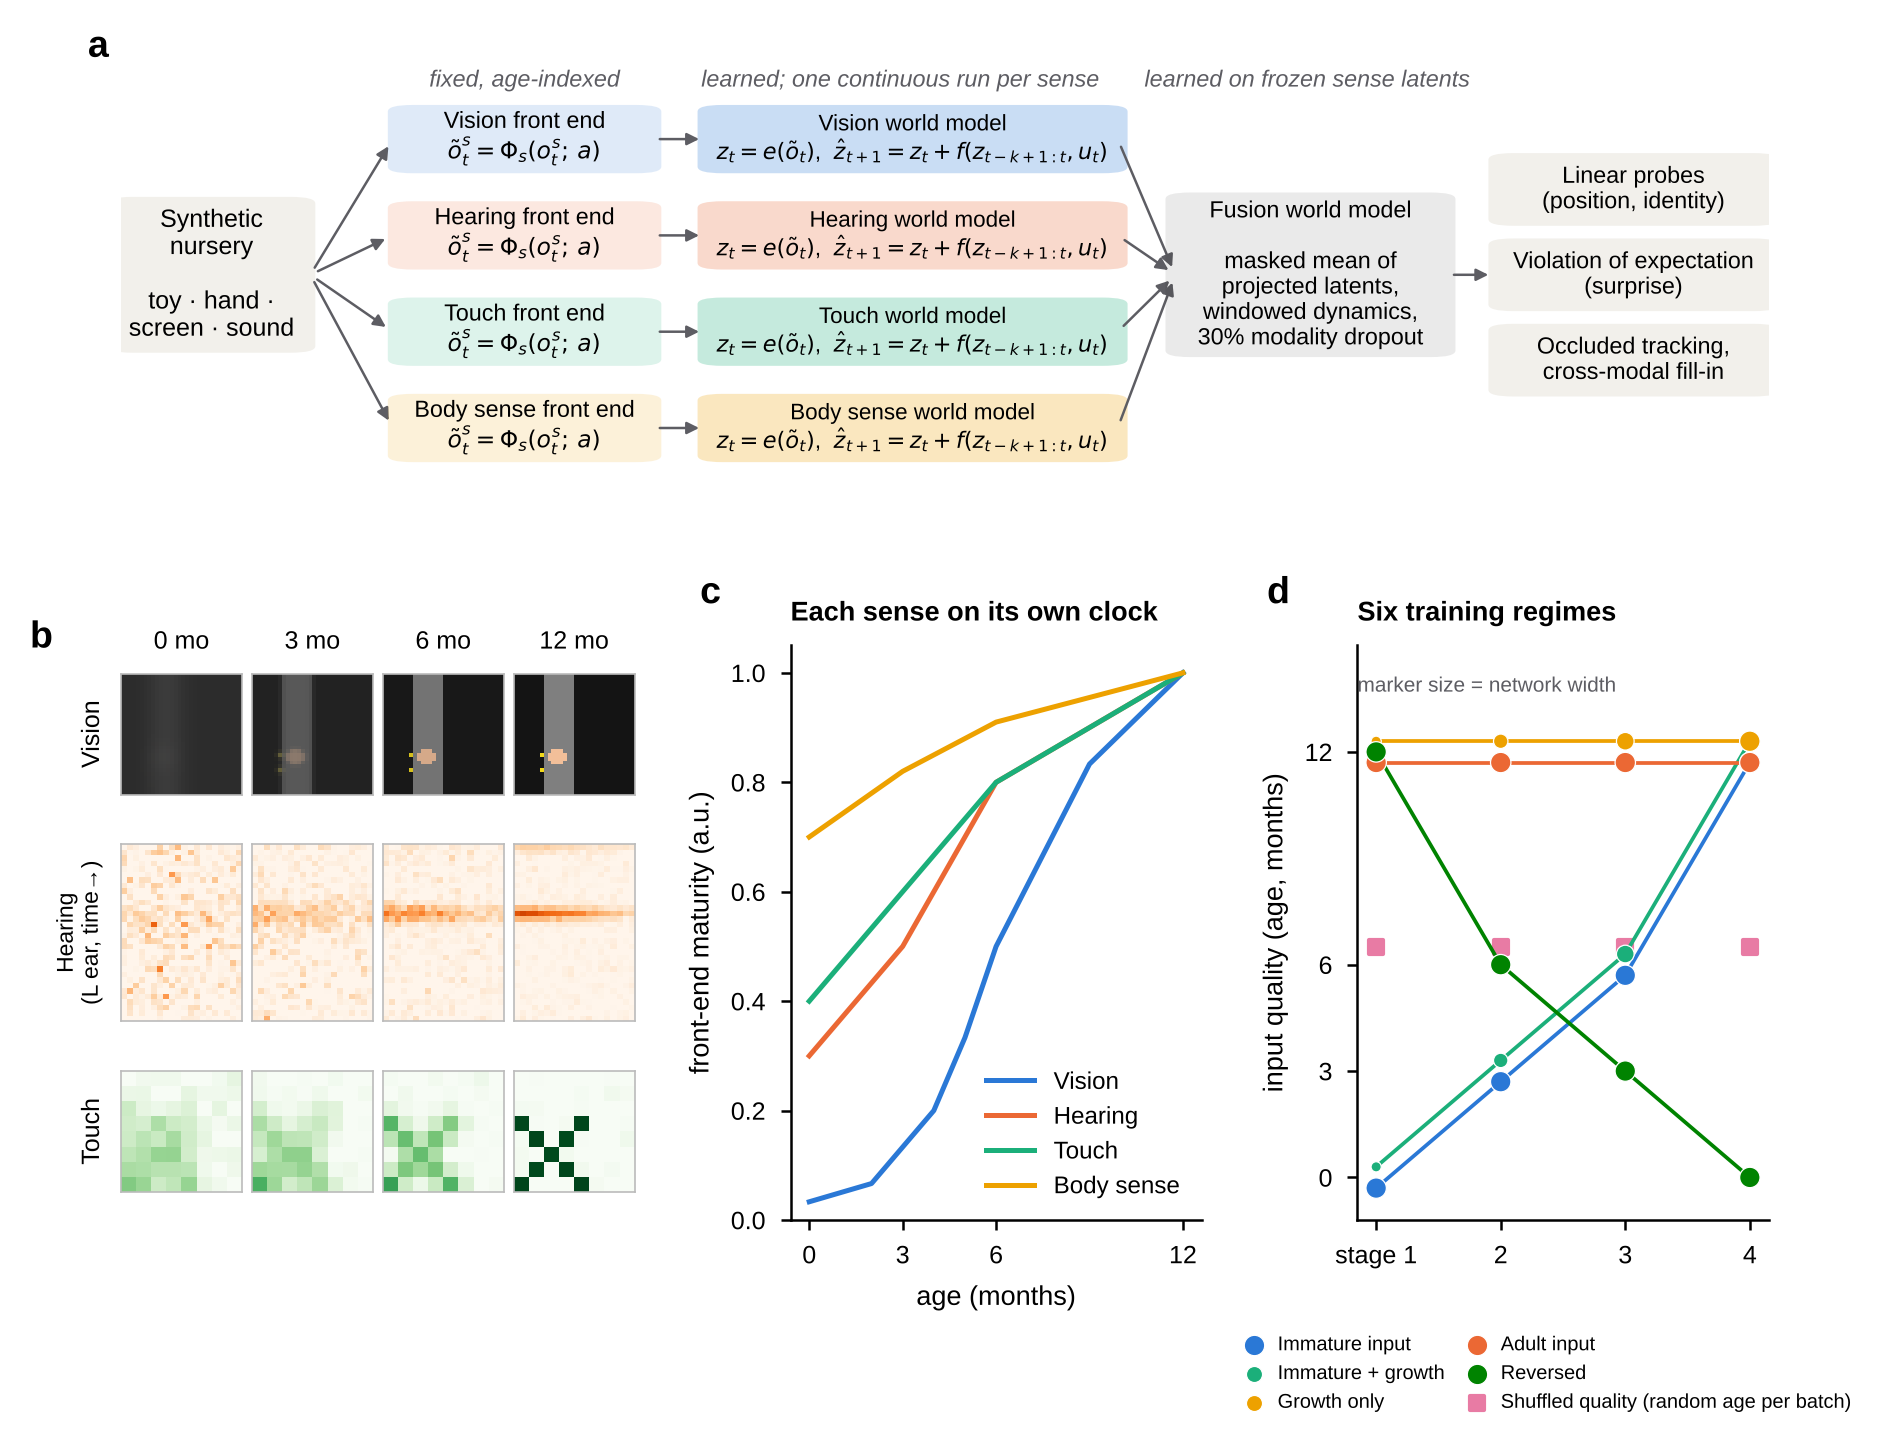
\includegraphics[width=1\textwidth,height=0.78\textheight,keepaspectratio]{fig1_overview.png}
\caption{\textbf{Architecture and curricula.} \textbf{a}, A synthetic scene (an object that is seen, heard and felt, an action-driven effector and an occluding screen) is passed through a fixed degradation operator \(\Phi_s(\cdot;a)\) per modality, and each modality learns its own world model: an encoder \(e\), a residual dynamics model \(f\) over the last \(k\) latents and the action \(u_t\), and a decoder. A fusion world model combines the frozen latents with a masked mean and 30\% modality dropout. Read-outs are linear probes, violation-of-expectation surprise and occluded tracking. \textbf{b}, The same frame delivered to vision, audio (left channel, 32 frequency bins over the episode) and touch (an \(8\times8\) patch) at stages \(a=0,3,6,12\). \textbf{c}, Operator maturity per modality (normalised parameters of Table~\ref{tab:frontends}). \textbf{d}, The six curricula: input quality over the four training stages; marker size is network width.}
\label{fig:overview}
\end{figure}

\subsection{Curricula and ablations}

Training proceeds in four stages of one continuous run, and the model is read out at the end of each stage. Six curricula (Table~\ref{tab:regimes}, Fig.~\ref{fig:overview}d) cross the input schedule with capacity. The degraded-to-clean schedule (\(a=0\to3\to6\to12\)) is the primary curriculum and is labelled ``Immature input'' in the figures; ``Adult input'' is the clean baseline (\(a=12\) throughout). Shuffled quality, which draws each batch from a random stage, separates the effect of having seen degraded input from the effect of its order, and the reversed schedule is a negative control. Growth widens every hidden layer at each stage boundary by function-preserving widening (Proposition~\ref{prop:growth}) and lengthens the memory window by adding zero input weights for the new slots, so the model's function is unchanged at each widening (checked numerically for every layer). Two further vision curricula ablate the operator: \emph{blur only} (acuity follows \(a\); contrast and colour clean) and \emph{contrast only} (contrast sensitivity follows \(a\); acuity and colour clean). All curricula see the same episodes, the same number of updates and the same hyperparameters, so any difference is due to the schedule or to growth.

\begin{longtable}[]{@{}
  >{\raggedright\arraybackslash}p{(\columnwidth - 4\tabcolsep) * \real{0.3333}}
  >{\raggedright\arraybackslash}p{(\columnwidth - 4\tabcolsep) * \real{0.3333}}
  >{\raggedright\arraybackslash}p{(\columnwidth - 4\tabcolsep) * \real{0.3333}}@{}}
\caption{Training curricula. All see the same episodes for the same number of updates. Names in quotation marks are the labels used in the figures.}\label{tab:regimes}\tabularnewline
\toprule\noalign{}
Curriculum & Network & Stage \(a\) across the four stages \\
\midrule\noalign{}
\endfirsthead
\toprule\noalign{}
Curriculum & Network & Stage \(a\) across the four stages \\
\midrule\noalign{}
\endhead
\bottomrule\noalign{}
\endlastfoot
Degraded-to-clean, ``Immature input'' (primary) & fixed (largest size) & 0 \ensuremath{\rightarrow} 3 \ensuremath{\rightarrow} 6 \ensuremath{\rightarrow} 12 \\
Degraded-to-clean + growth, ``Immature + growth'' & grows \ensuremath{\times}1 \ensuremath{\rightarrow} \ensuremath{\times}4 & 0 \ensuremath{\rightarrow} 3 \ensuremath{\rightarrow} 6 \ensuremath{\rightarrow} 12 \\
Growth only & grows \ensuremath{\times}1 \ensuremath{\rightarrow} \ensuremath{\times}4 & 12 throughout \\
Clean baseline, ``Adult input'' & fixed & 12 throughout \\
Shuffled quality & fixed & each batch from a random stage \\
Reversed & fixed & 12 \ensuremath{\rightarrow} 6 \ensuremath{\rightarrow} 3 \ensuremath{\rightarrow} 0 \\
\end{longtable}

\subsection{Evaluation}

\textbf{Linear probes.} We judge a model's internal state with a ridge-regression probe fitted on training episodes and scored on test episodes by \(R^2\), the fraction of a quantity's variance the probe recovers (0 is no better than the mean, 1 is perfect); identity uses one-hot targets and the arg-max (chance 0.25). A probe measures what is stored, not what the network does with it. \emph{Clean} probes are fitted and tested on \(a=12\) input; \emph{own-stage} probes on the input of the checkpoint's stage; \emph{stage-0} probes are fitted on clean input and tested on \(a=0\) input.

\textbf{Information ceiling.} For each modality and stage we train a separate supervised network, with the encoder design of the world models, directly on single filtered frames to regress the object's position and classify its identity. Its held-out score estimates the best score reachable from that stage's input.

\textbf{Violation of expectation.} Surprise is the squared error of the one-step forecast, \(S_t=\lVert d(\hat z_t)-\tilde o_t\rVert^2\) for a modality model or \(\lVert r_s(\hat h_t)-z^s_t\rVert^2\) per channel for the fused model, averaged over the occluded stretch and the two frames after expected re-emergence. Paired \emph{possible} events (the object passes behind a screen and reappears) and \emph{impossible} events (it vanishes while hidden) share all random draws. The index
\begin{equation}\mathrm{VoE}=\frac{S_{\text{imp}}-S_{\text{pos}}}{S_{\text{imp}}+S_{\text{pos}}}\in[-1,1]\label{eq:voe}\end{equation}
is positive when the impossible event is the more surprising. Two dissociating events remove the object from vision and touch while it keeps sounding, or remove a silent object.

\textbf{Occluded tracking and fill-in.} The occluded object's horizontal position is probed on fully hidden frames from the vision model's memory window (\(k=6\) latents), from the audio latent and from the fused state. Fill-in probes position from the fused state with all modalities, with vision masked, and from single modalities.

\section{Theory}
\label{sec:theory}

We state four results about the setting of Section~\ref{sec:model}. Each proof is short and given in full; Fig.~\ref{fig:theory} and Section~\ref{sec:results} test each result.

\begin{proposition}[Information bound]\label{prop:info}
Let \(Y\) be a scene property, \(O\) the clean observation and \(\tilde O_a=\Phi(O;a)\) the filtered observation, with \(\Phi\) a stochastic degradation of \(O\), so that \(Y\to O\to\tilde O_a\) is a Markov chain. Then for every representation \(Z=e(\tilde O_a)\),
\begin{equation}I(Z;Y)\le I(\tilde O_a;Y)\le I(O;Y),\end{equation}
and the best squared-error read-out has ceiling \(R^2_\star(a)=1-\mathbb E[\operatorname{Var}(Y\mid\tilde O_a)]/\operatorname{Var}(Y)\), which does not increase from stage \(a\) to stage \(a'\) whenever \(\tilde O_{a'}\) is a further degradation of \(\tilde O_a\) (nested operators, so that \(Y\to\tilde O_a\to\tilde O_{a'}\) is a Markov chain).
\end{proposition}

\begin{proof}
The inequalities are the data-processing inequality applied twice. For the ceiling, if \(\tilde O_{a'}\) is a further degradation of \(\tilde O_a\) then \(\mathbb E[Y\mid\tilde O_{a'}]=\mathbb E\big[\mathbb E[Y\mid\tilde O_a]\mid\tilde O_{a'}\big]\), and by Jensen's inequality the variance of this conditional mean cannot exceed that of \(\mathbb E[Y\mid\tilde O_a]\). Since \(\operatorname{Var}(Y)=\mathbb E\operatorname{Var}(Y\mid\cdot)+\operatorname{Var}(\mathbb E[Y\mid\cdot])\), the residual variance cannot decrease.
\end{proof}

The proposition separates what the input contains from what learning extracts. The supervised ceiling we report estimates \(R^2_\star(a)\) from below; the gap between a self-supervised model and that ceiling is a property of learning.

\begin{proposition}[Learning time under gradient flow]\label{prop:time}
Let \(\tilde x=\Phi(o;a)-\mathbb E\,\Phi(o;a)\) be the centred filtered input, \(y\) a standardised target, \(\Sigma=\mathbb E\,\tilde x\tilde x^\top=\sum_i\lambda_i v_iv_i^\top\) its covariance and \(c_i=v_i^\top\mathbb E[\tilde x y]\). A linear read-out with \(W(0)=0\) trained by gradient flow \(\dot W=-\nabla_W\mathbb E\lVert y-W^\top\tilde x\rVert^2/2\) has explained variance
\begin{equation}R^2(t)=\sum_{i:\lambda_i>0}\frac{c_i^2}{\lambda_i}\Big(1-e^{-2\lambda_i t}\Big),\qquad R^2(\infty)=\sum_{i:\lambda_i>0}\frac{c_i^2}{\lambda_i}.\label{eq:r2t}\end{equation}
Consequently: (a) if the operator scales input fluctuations by \(\kappa\), then \(\lambda_i\to\kappa^2\lambda_i\) and \(c_i\to\kappa c_i\), so \(R^2_\kappa(t)=R^2_1(\kappa^2t)\): the same ceiling is reached \(\kappa^{-2}\) times later. (b) If the operator is a Gaussian blur with standard deviation \(\sigma\) and the input statistics are approximately shift-invariant, the variance of a mode at angular spatial frequency \(\omega\) is multiplied by \(e^{-\sigma^2\omega^2}\), so its learning time is multiplied by \(e^{\sigma^2\omega^2}\): coarse modes are barely affected, fine modes are learned exponentially later, and modes whose variance falls below a noise floor or the resolution of a finite training budget are not learned at all.
\end{proposition}

\begin{proof}
In the eigenbasis of \(\Sigma\) the modes decouple: \(\dot w_i=c_i-\lambda_iw_i\), so \(w_i(t)=(c_i/\lambda_i)(1-e^{-\lambda_it})\). The variance explained by mode \(i\) is \(2w_ic_i-\lambda_iw_i^2=(c_i^2/\lambda_i)(1-e^{-2\lambda_it})\), and the modes add. For (a), scaling \(\tilde x\) by \(\kappa\) scales \(\Sigma\) by \(\kappa^2\) and the cross-covariance by \(\kappa\), so \(c_i^2/\lambda_i\) is unchanged and \(\lambda_it\) becomes \(\kappa^2\lambda_it\). For (b), the Fourier transform of a Gaussian of width \(\sigma\) is \(e^{-\sigma^2\omega^2/2}\), so power at frequency \(\omega\) is multiplied by \(e^{-\sigma^2\omega^2}\).
\end{proof}

Two points limit how far this carries. The statement is for a linear read-out and plain gradient descent; deep linear networks show a similar inverse dependence of learning time on the strength of an input--output mode, with sigmoidal rather than exponential timing \autocite{saxe2019mathematical}, and nonlinear networks can only be expected to follow it loosely. And adaptive optimisers such as Adam \autocite{kingma2015adam} divide each step by a running estimate of gradient magnitude, which weakens the dependence on the global scale \(\kappa\) (for a linear read-out, from \(\kappa^{-2}\) towards roughly \(\kappa^{-1}\)); whether contrast or blur dominates in a trained network is therefore an empirical question, which the operator ablations answer.

\begin{proposition}[Growth delay]\label{prop:growth}
Widen a hidden layer from \(n\) to \(n'\) units by \(W_1'=\begin{bmatrix}W_1\\R\end{bmatrix}\) and \(W_2'=[\,W_2\;\;0\,]\), with \(R\) arbitrary. Then the network's function is unchanged, \(W_2'\phi(W_1'x)=W_2\phi(W_1x)\), and the gradient on the new incoming weights is zero,
\begin{equation}\frac{\partial\mathcal L}{\partial R}=\big(\mathbf 0^\top\delta\big)\odot\phi'(Rx)\,x^\top=0,\end{equation}
while the gradient on the new outgoing weights \(A\) (initially \(0\)) is \(\partial\mathcal L/\partial A=\mathbb E\big[\delta\,\phi(Rx)^\top\big]\), which is nonzero only if the new units' activations are correlated with the residual error \(\delta\) (for \(\phi(0)=0\) this requires \(R\neq0\)). New capacity therefore starts to learn only through its outgoing weights: once \(A\neq0\) the new units act as fixed random features, and their incoming weights \(R\) adapt at a rate proportional to \(\lVert A\rVert\).
\end{proposition}

\begin{proof}
The first claim follows because the new units' contribution is multiplied by zero. The gradient with respect to \(R\) passes through the new outgoing weights \(0\), which gives the displayed expression. The gradient with respect to the new outgoing weights is \(\mathbb E[\delta\,\phi(Rx)^\top]\), which is nonzero unless \(\phi(Rx)\) is uncorrelated with the residual.
\end{proof}

The origin \((r,a)=(0,0)\) of one incoming and one outgoing weight is a saddle of the loss. With \(\dot a=\rho r\) and \(\dot r=\rho a\), where \(\rho\) measures the correlation of the new unit with the residual, \(a(t)=a_0\cosh\rho t+r_0\sinh\rho t\), so \(a\) reaches a given size \(a^\ast\) after \(t\approx\rho^{-1}\log\big(2a^\ast/\lvert a_0+r_0\rvert\big)\): with \(a_0=0\) the delay grows with \(\log(1/\lvert r_0\rvert)\) and shrinks with \(\rho\), which itself falls as the existing units absorb the residual. (Here \(a\) denotes an outgoing weight, not a stage.) This is the zero-outgoing-weight variant of function-preserving widening; Net2Net instead copies existing units and divides their outgoing weights among the copies \autocite{chen2016net2net}, which also preserves the function but does not start the new units at this saddle. Growth of this kind therefore buys a cheaper early network (fewer parameter-updates) at the price of a plateau after each widening.

\begin{proposition}[Surprise of a squared-error forecaster]\label{prop:surprise}
The predictor \(\hat o_{t+1}\) minimising \(\mathbb E\lVert\hat o_{t+1}-o_{t+1}\rVert^2\) given the past is the conditional mean \(\mathbb E[o_{t+1}\mid o_{\le t}]\). Consider a pixel behind a screen, which shows \(o^{\text{obj}}\) if the object reappears at the next frame, with probability \(p\), and \(o^{\text{screen}}\) otherwise, and let \(\Delta=o^{\text{obj}}-o^{\text{screen}}\neq0\). The optimal forecast is \((1-p)\,o^{\text{screen}}+p\,o^{\text{obj}}\) and the surprise (squared error) is
\begin{equation}S_{\text{reappear}}=(1-p)^2\Delta^2,\qquad S_{\text{vanish}}=p^2\Delta^2 .\end{equation}
The forecaster is more surprised by reappearance than by non-reappearance exactly when \(p<\tfrac12\).
\end{proposition}

\begin{proof}
The conditional mean minimises mean squared error (by the decomposition \(\mathbb E\lVert\hat o-o\rVert^2=\mathbb E\lVert\hat o-\mathbb E[o\mid\cdot]\rVert^2+\mathbb E\operatorname{tr}\operatorname{Cov}(o\mid\cdot)\)). Substituting the two outcomes gives the displayed errors, with \(\Delta^2\) read as \(\lVert\Delta\rVert^2\) for vector observations.
\end{proof}

When the time of reappearance is uncertain, \(p<\tfrac12\) for most frames of an occlusion, so a negative violation-of-expectation index (\ref{eq:voe}), averaged over frames, is the correct behaviour of a well-trained pixel forecaster and is not a failure of training or of memory. The argument is exact for the unweighted loss; with extra weight \(w_r\ge1\) on moving pixels, as in (\ref{eq:loss}), the threshold \(\tfrac12\) becomes \(1/(1+w_r)\). A positive index requires either a forecaster whose probability of reappearance exceeds that threshold, or an additional signal (such as a sound) that makes the impossible event informative.

Fig.~\ref{fig:theory} shows the spectral quantities of Proposition~\ref{prop:time} measured on the environment's own frames.

\begin{figure}[htbp]
\centering
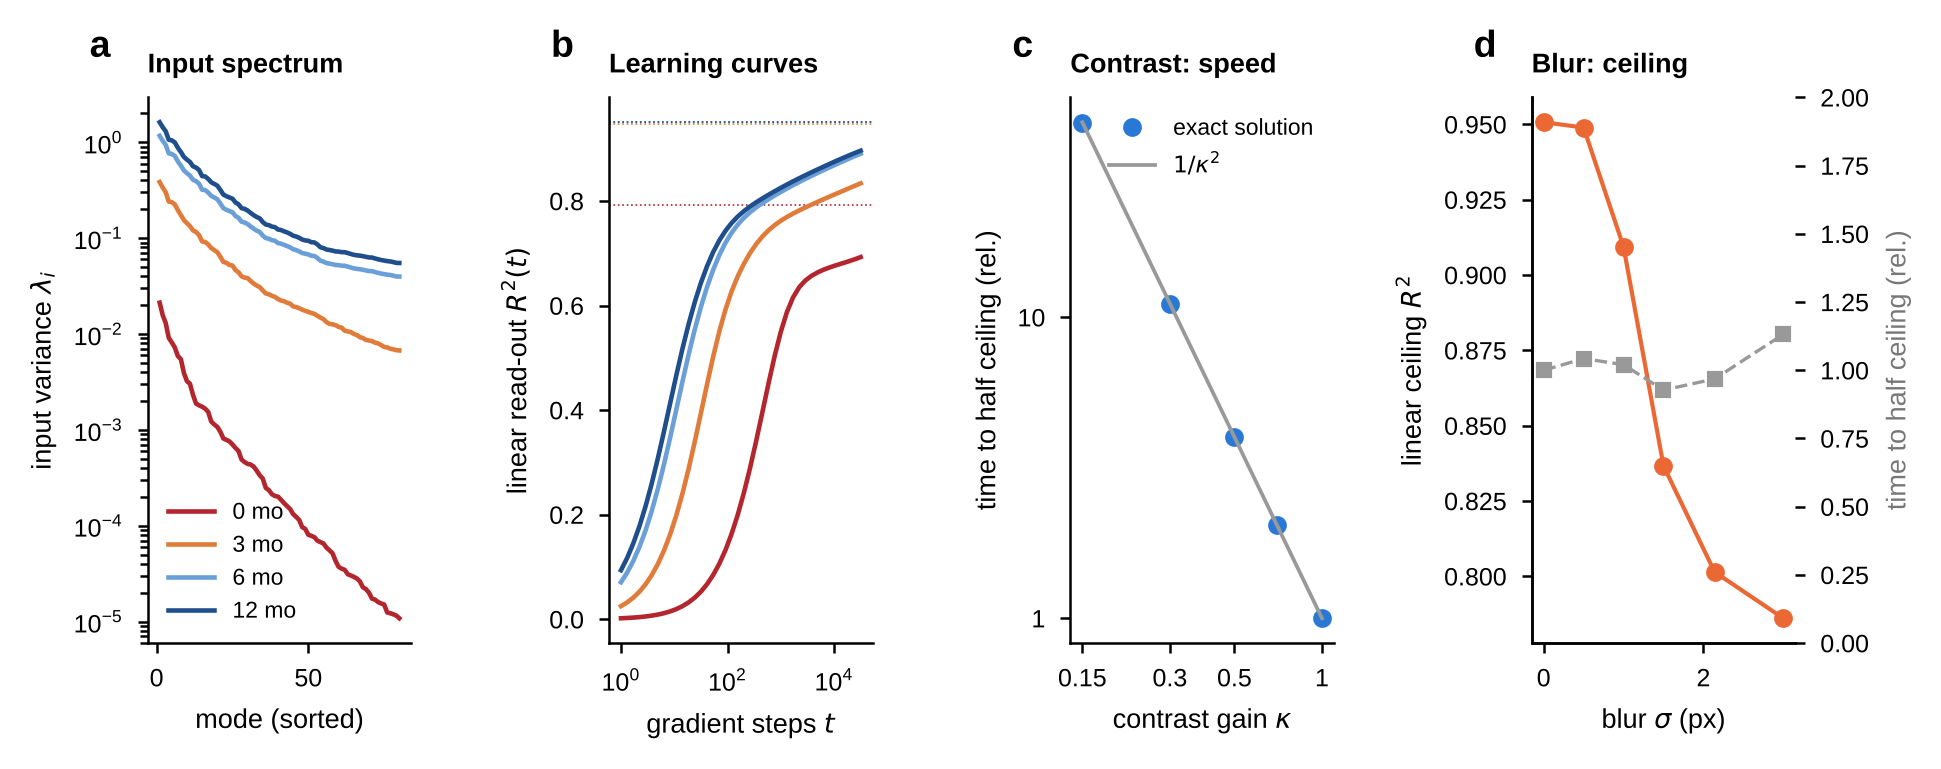
\includegraphics[width=1\textwidth,height=0.78\textheight,keepaspectratio]{fig6_theory.png}
\caption{\textbf{Spectral account of learning time.} For the object-position read-out from filtered frames. \textbf{a}, Eigenvalue spectrum of the input covariance at the four stages: degraded operators shrink it by orders of magnitude. \textbf{b}, Exact gradient-flow solution \(R^2(t)\) of Proposition~\ref{prop:time} for each stage with the step size fixed by the clean input; dotted lines, the linear ceilings. \textbf{c}, Time to half the ceiling when only contrast is scaled by \(\kappa\): the exact solution follows \(\kappa^{-2}\). \textbf{d}, Blur alone: the ceiling falls with the blur width while the time to half ceiling barely moves.}
\label{fig:theory}
\end{figure}

\section{Results}
\label{sec:results}

\textbf{Setup.} The environment renders one object of four types, an action-driven effector and, in half the scenes, a vertical screen into four streams: \(32\times32\) colour vision, binaural audio (2 channels \ensuremath{\times} 32 frequency bins, panned by position and passing through the screen), an \(8\times8\) tactile patch on the effector, and four-dimensional proprioception (Fig.~\ref{fig:overview}a; Appendix~\ref{app:env}). Each object type is specified redundantly across modalities, by shape and colour, pitch and felt shape \autocite{bahrick2000intersensory}. Each modality is trained in one continuous run of four stages and read out at the end of each. Results are mean \(\pm\) s.d. over 5 seeds per curriculum; the stage labels \(a=0,3,6,12\) appear in the figures as months.

\textbf{Under the degraded-to-clean curriculum, vision learns late and slowly.} The vision model cannot localise the object at the first checkpoint (position \(R^2\) 0.02 \ensuremath{\pm} 0.00) and is still poor at the second (0.31 \ensuremath{\pm} 0.15), then rises to 0.85 \ensuremath{\pm} 0.04 (Fig.~\ref{fig:development}a). Trained on clean input the same network localises the object from the first checkpoint (0.69 \ensuremath{\pm} 0.04) and ends at 0.89 \ensuremath{\pm} 0.03. The audio, tactile and proprioceptive models are close to their final level much earlier (Fig.~\ref{fig:development}c, e), an order set by the operator tables.

\begin{figure}[htbp]
\centering
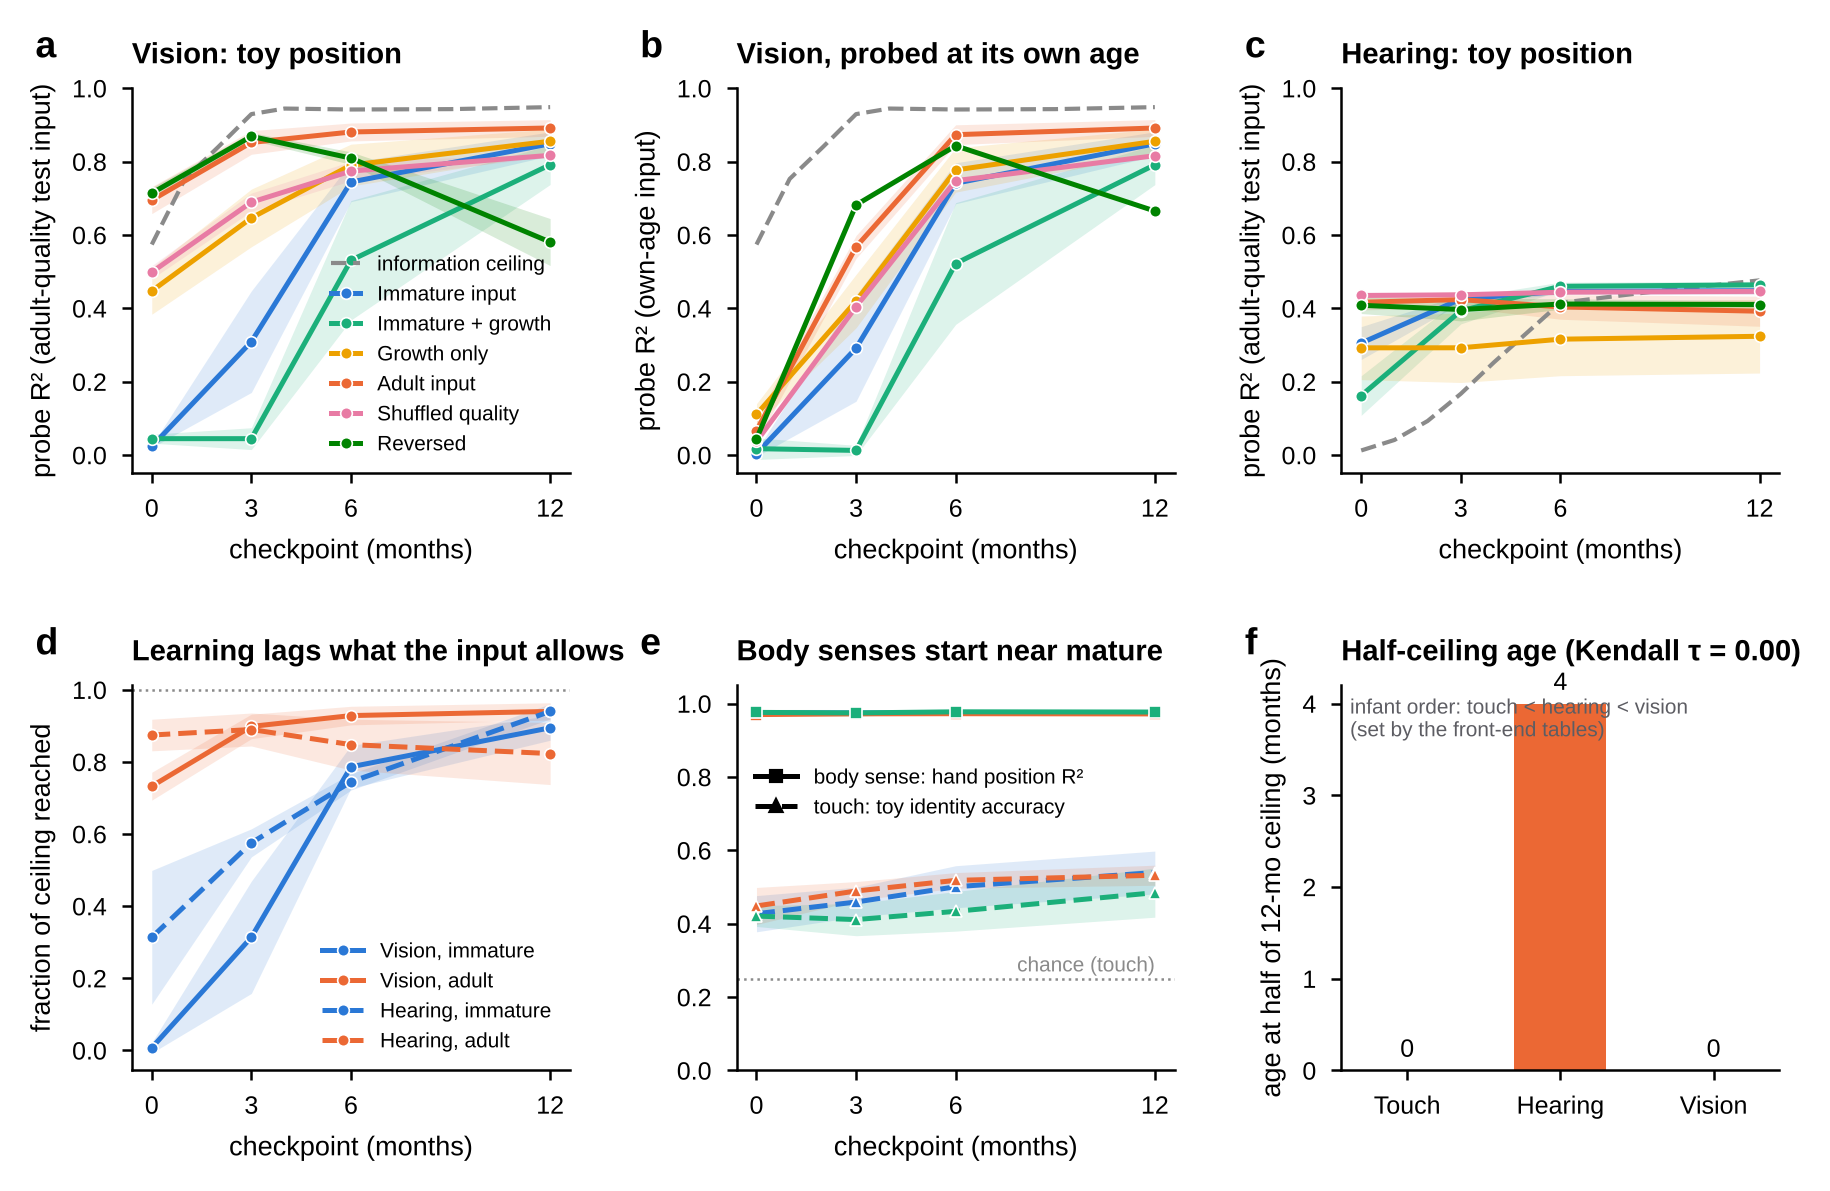
\includegraphics[width=1\textwidth,height=0.78\textheight,keepaspectratio]{fig2_development.png}
\caption{\textbf{Learning curves per modality and curriculum.} Checkpoints are labelled by stage \(a\) in months. The ceiling and own-stage data for vision and audio are also plotted in the companion paper \autocite{mohapatra2026senses}. \textbf{a}, Object position decoded from the vision model's latent at each checkpoint (clean probe), for the six curricula; dashed grey line, information ceiling (a supervised network trained directly on that stage's filtered input). \textbf{b}, The same with the own-stage probe. \textbf{c}, Audio. \textbf{d}, Fraction of the stage-matched ceiling reached by the degraded-to-clean curriculum (own-stage probe) and by the clean baseline, for vision (solid) and audio (dashed). \textbf{e}, Proprioception (effector position \(R^2\), squares) and touch (object identity accuracy, triangles; chance 0.25). \textbf{f}, Stage at which each modality's information ceiling first reaches half its final value, compared with the biological order of maturation (Appendix~\ref{app:milestones}). Lines, mean over seeds; bands, \ensuremath{\pm}1 s.d.; n = 5 seeds per curriculum.}
\label{fig:development}
\end{figure}

\textbf{The early failure is a property of learning, not of the input.} Proposition~\ref{prop:info} separates the two. Probing on each checkpoint's own input (Fig.~\ref{fig:development}b) gives 0.00 \ensuremath{\pm} 0.01 at \(a=0\) and 0.85 \ensuremath{\pm} 0.04 at \(a=12\), so the failure is not a distribution shift from training on degraded and testing on clean images. The \(a=0\) input is not empty: a supervised network trained directly on it reaches \(R^2\) = 0.60 (Fig.~\ref{fig:development}a, dashed), and the exact linear solution of Proposition~\ref{prop:time} reaches 0.79. The gap between 0.60 and 0.02 is therefore a property of learning. Proposition~\ref{prop:time} quantifies it for the linear read-out: with the step size set by clean input, the \(a=0\) operator shrinks the total input variance from 32.20 to 0.12 and lengthens the time to half ceiling 39-fold (Fig.~\ref{fig:theory}a, b). The vision model approaches its ceiling only as the operator sharpens (Fig.~\ref{fig:development}d).

\textbf{In the linear model, contrast sets the speed of learning and blur sets the ceiling.} Scaling contrast alone by \(\kappa\) delays the linear solution by \(\kappa^{-2}\) to within 1\% over a 44-fold range and leaves its ceiling unchanged (Fig.~\ref{fig:theory}c). Blur alone leaves the time to half ceiling almost unchanged but lowers the ceiling from 0.95 without blur to 0.80 at the \(a=0\) width of 2.14 px (Fig.~\ref{fig:theory}d). The linear read-out is not the network, and the networks are trained with Adam, which weakens the global scale effect; the operator ablations test which component matters in the trained vision model.

\textbf{In the trained network, contrast, not blur, produces the early lag.} When only blur follows the curriculum, the vision model already localises the object at the first checkpoint (0.34 \ensuremath{\pm} 0.05, against 0.69 \ensuremath{\pm} 0.04 for clean input and 0.02 \ensuremath{\pm} 0.00 for the full curriculum), reaches 0.79 \ensuremath{\pm} 0.05 at the second and ends at 0.88 \ensuremath{\pm} 0.02 (Fig.~\ref{fig:ablation}a). When only contrast follows the curriculum, the model reproduces the full lag (0.04 \ensuremath{\pm} 0.02 at the first checkpoint, 0.51 \ensuremath{\pm} 0.04 at the second), and identity accuracy follows the same pattern (0.37 \ensuremath{\pm} 0.03 against 0.60 \ensuremath{\pm} 0.06 for blur only at the second checkpoint; Fig.~\ref{fig:ablation}b). Contrast therefore accounts for nearly all of the early delay, as Proposition~\ref{prop:time} predicts, even under Adam; blur alone costs little speed at this image scale. Colour saturation was held at the clean value in both ablations, so its contribution is untested.

\begin{figure}[htbp]
\centering
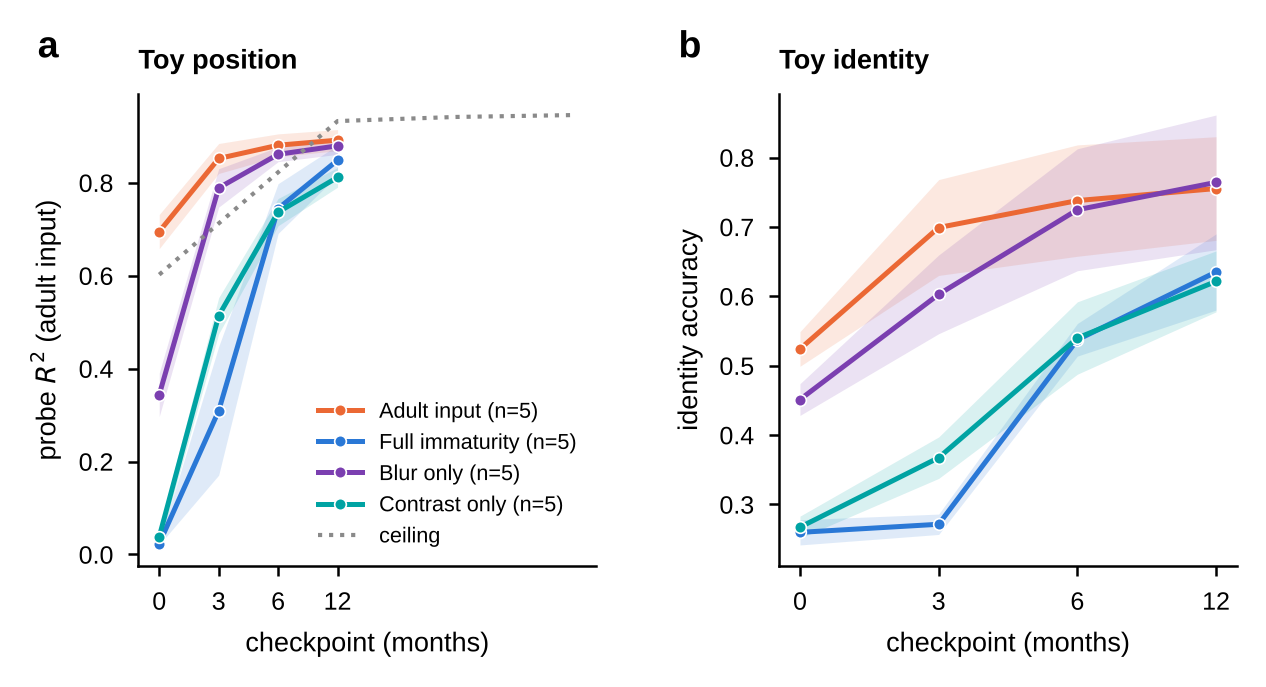
\includegraphics[width=0.7\textwidth,height=0.78\textheight,keepaspectratio]{fig7_ablation.png}
\caption{\textbf{Operator ablations in the trained vision model.} Vision probe score (\textbf{a}, object position; \textbf{b}, object identity; clean test input) at the four checkpoints for clean input (``Adult input''), the full degraded-to-clean curriculum, and curricula in which only blur or only contrast follows the stage (colour is clean in both). Lines, mean over seeds; bands, \ensuremath{\pm}1 s.d.; n = 5 seeds per curriculum.}
\label{fig:ablation}
\end{figure}

\textbf{Trained encoders respond first to the coarse, high-variance input modes and widen as the operator sharpens.} To ask whether the spectral account carries over to trained networks, we measured the Jacobian of each vision encoder on clean frames and expressed it in the eigenbasis of the clean input covariance (Extended Data Fig.~S4c, d). At the first checkpoint the degraded-to-clean encoder puts 0.52 \ensuremath{\pm} 0.09 of its Jacobian energy in the ten input modes that carry 0.69 of the input variance, against 0.09 \ensuremath{\pm} 0.01 for the encoder trained on clean input throughout, and its effective rank is 4.3 \ensuremath{\pm} 0.6 against 12.9 \ensuremath{\pm} 0.8. The share falls and the rank rises as the operator sharpens (0.06 \ensuremath{\pm} 0.02 and 13.5 \ensuremath{\pm} 1.2 at \(a=12\)), but the rank stays below that of the clean-input encoder (17.9 \ensuremath{\pm} 1.0). Early learning from degraded input is therefore concentrated on the modes that dominate the input, as Proposition~\ref{prop:time} implies for a linear read-out, and the fine modes are acquired later. This is a measurement on the encoder, not on the map to the object's position, and it supports the spectral account without proving it for deep networks.

\textbf{Growth delays learning and halves the parameter-updates.} Adding growth to the degraded-to-clean curriculum does not change the shape of the curve; it delays it (Fig.~\ref{fig:development}a). The grown vision model is still at \(R^2\) 0.04 \ensuremath{\pm} 0.03 at the \(a=3\) checkpoint and ends at 0.79 \ensuremath{\pm} 0.06, against 0.85 \ensuremath{\pm} 0.04 for the fixed-size network; identity accuracy is 0.49 \ensuremath{\pm} 0.06 against 0.64 \ensuremath{\pm} 0.06 (Hedges' \(g\) = \ensuremath{-}2.2, \(p\) = 0.005). Growth on clean input learns quickly and ends near the clean baseline (0.86 \ensuremath{\pm} 0.04). Growing networks use 0.48 of the fixed network's parameter-updates (Fig.~\ref{fig:costs}d). This is the plateau Proposition~\ref{prop:growth} predicts: new units begin learning only through their outgoing weights, so each widening is followed by a stall, and growth trades accuracy for compute.

\begin{figure}[htbp]
\centering
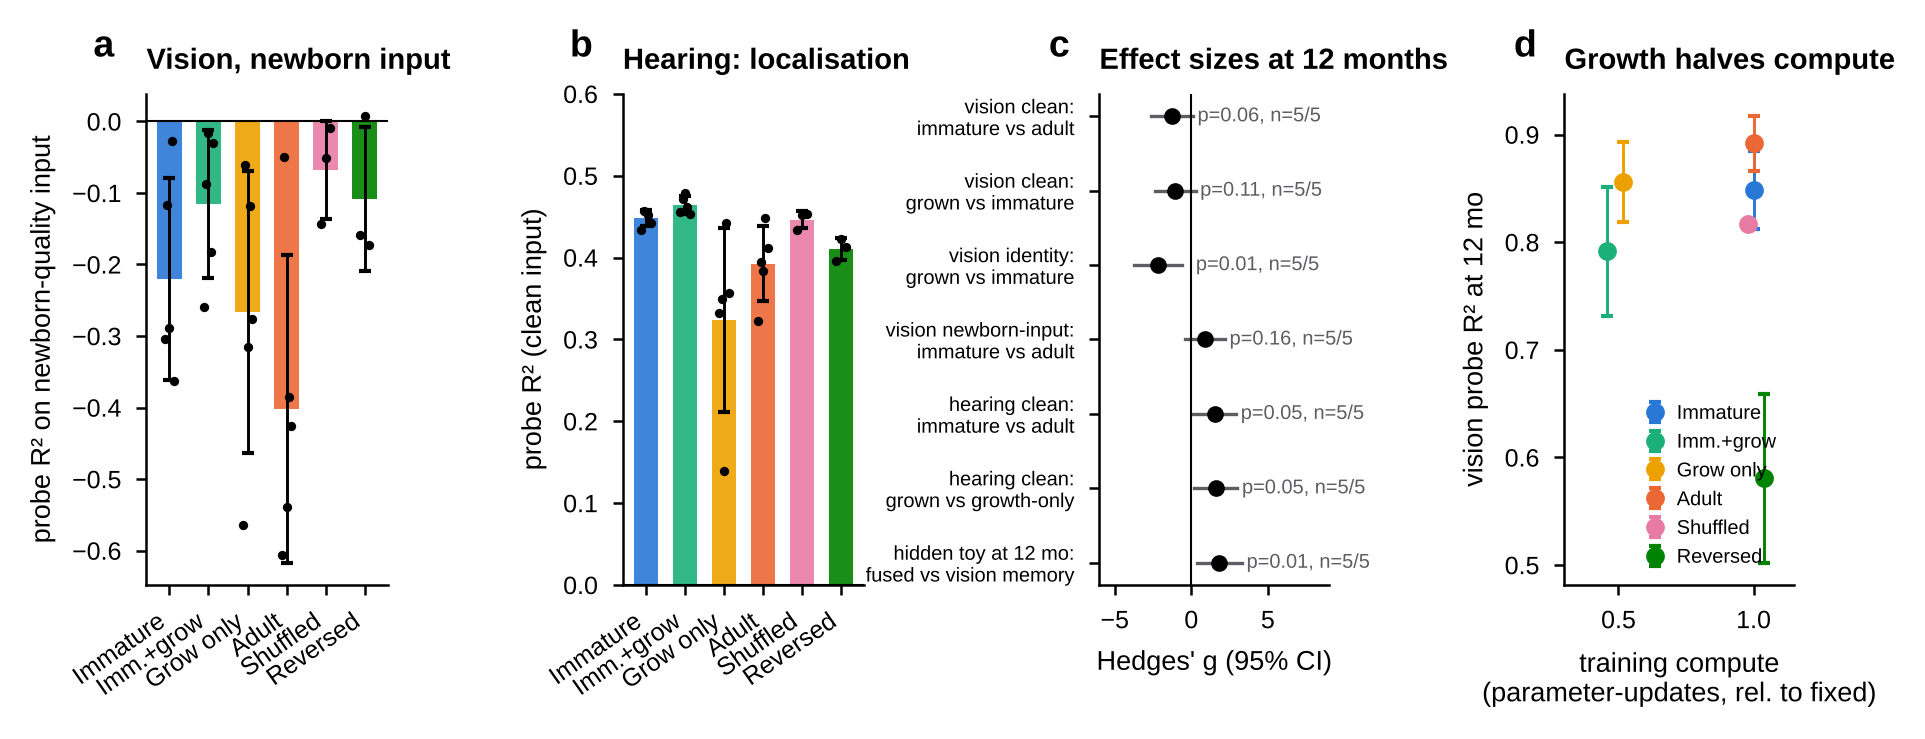
\includegraphics[width=1\textwidth,height=0.78\textheight,keepaspectratio]{fig3_costs_benefits.png}
\caption{\textbf{Costs and benefits at the final checkpoint (\(a=12\)).} \textbf{a}, Vision probe \(R^2\) when tested on \(a=0\) input (bars, mean; dots, seeds; whiskers, s.d.). All values are negative (worse than predicting the mean), so differences are in how badly models fail. \textbf{b}, Audio localisation on clean input. \textbf{c}, Effect sizes (Hedges' \(g\) with approximate 95\% CI) and Welch-test \(p\) values for the planned comparisons; n per group shown. \textbf{d}, Vision accuracy against training compute (parameter-updates relative to a fixed-size network).}
\label{fig:costs}
\end{figure}

\textbf{The degraded-to-clean curriculum costs vision a little.} On clean input the clean-baseline vision model is best; the curriculum costs 0.89 \ensuremath{-} 0.85 in \(R^2\) (\(g\) = \ensuremath{-}1.2, \(p\) = 0.06). Tested on \(a=0\) input, every model fails (Fig.~\ref{fig:costs}a), with curricula that included degraded input failing less on average (\ensuremath{-}0.22 \ensuremath{\pm} 0.14 against \ensuremath{-}0.40 \ensuremath{\pm} 0.22 for clean input), but the difference is within seed variability (\(p\) = 0.16); we do not claim a robustness benefit in vision.

\textbf{Degraded audio early helps localisation, mainly as augmentation.} Audio models that received degraded input early localise better on clean input at the final checkpoint (0.45 \ensuremath{\pm} 0.01 degraded-to-clean, 0.46 \ensuremath{\pm} 0.01 with growth) than models that only received clean input (0.39 \ensuremath{\pm} 0.05 clean baseline, 0.32 \ensuremath{\pm} 0.11 growth only; Fig.~\ref{fig:costs}b; \(g\) = 1.5, \(p\) = 0.05). Shuffled quality (0.44 \ensuremath{\pm} 0.01) is close to the ordered curriculum, so the benefit comes from having seen degraded input at all, a form of data augmentation, more than from its order. The reversed curriculum is the clearest negative control: the vision model that ends on \(a=0\) input falls from 0.85 \ensuremath{\pm} 0.04 to 0.59 \ensuremath{\pm} 0.07, so what it has learned does not survive a late degradation.

\textbf{Fusion with modality masking recovers what each modality alone loses.} During a long occlusion, the hidden object's horizontal position can be decoded from the vision model's memory (\(R^2\) 0.60 \ensuremath{\pm} 0.08 at the final checkpoint), from audio, which passes through the screen (0.42 \ensuremath{\pm} 0.09), and best from the fused world model (0.75 \ensuremath{\pm} 0.06; Fig.~\ref{fig:fusion}a; the paired difference fused minus vision is positive in every seed). The advantage appears at \(a=6\), and nothing is decodable at \(a=0\) to 3, when neither vision nor binaural audio can localise. For a visible object, the fused state is better than vision alone (0.87 \ensuremath{\pm} 0.03 against 0.79 \ensuremath{\pm} 0.06) and, with vision masked, still recovers position from audio, touch and proprioception (0.53 \ensuremath{\pm} 0.01; Fig.~\ref{fig:fusion}b).

\begin{figure}[htbp]
\centering
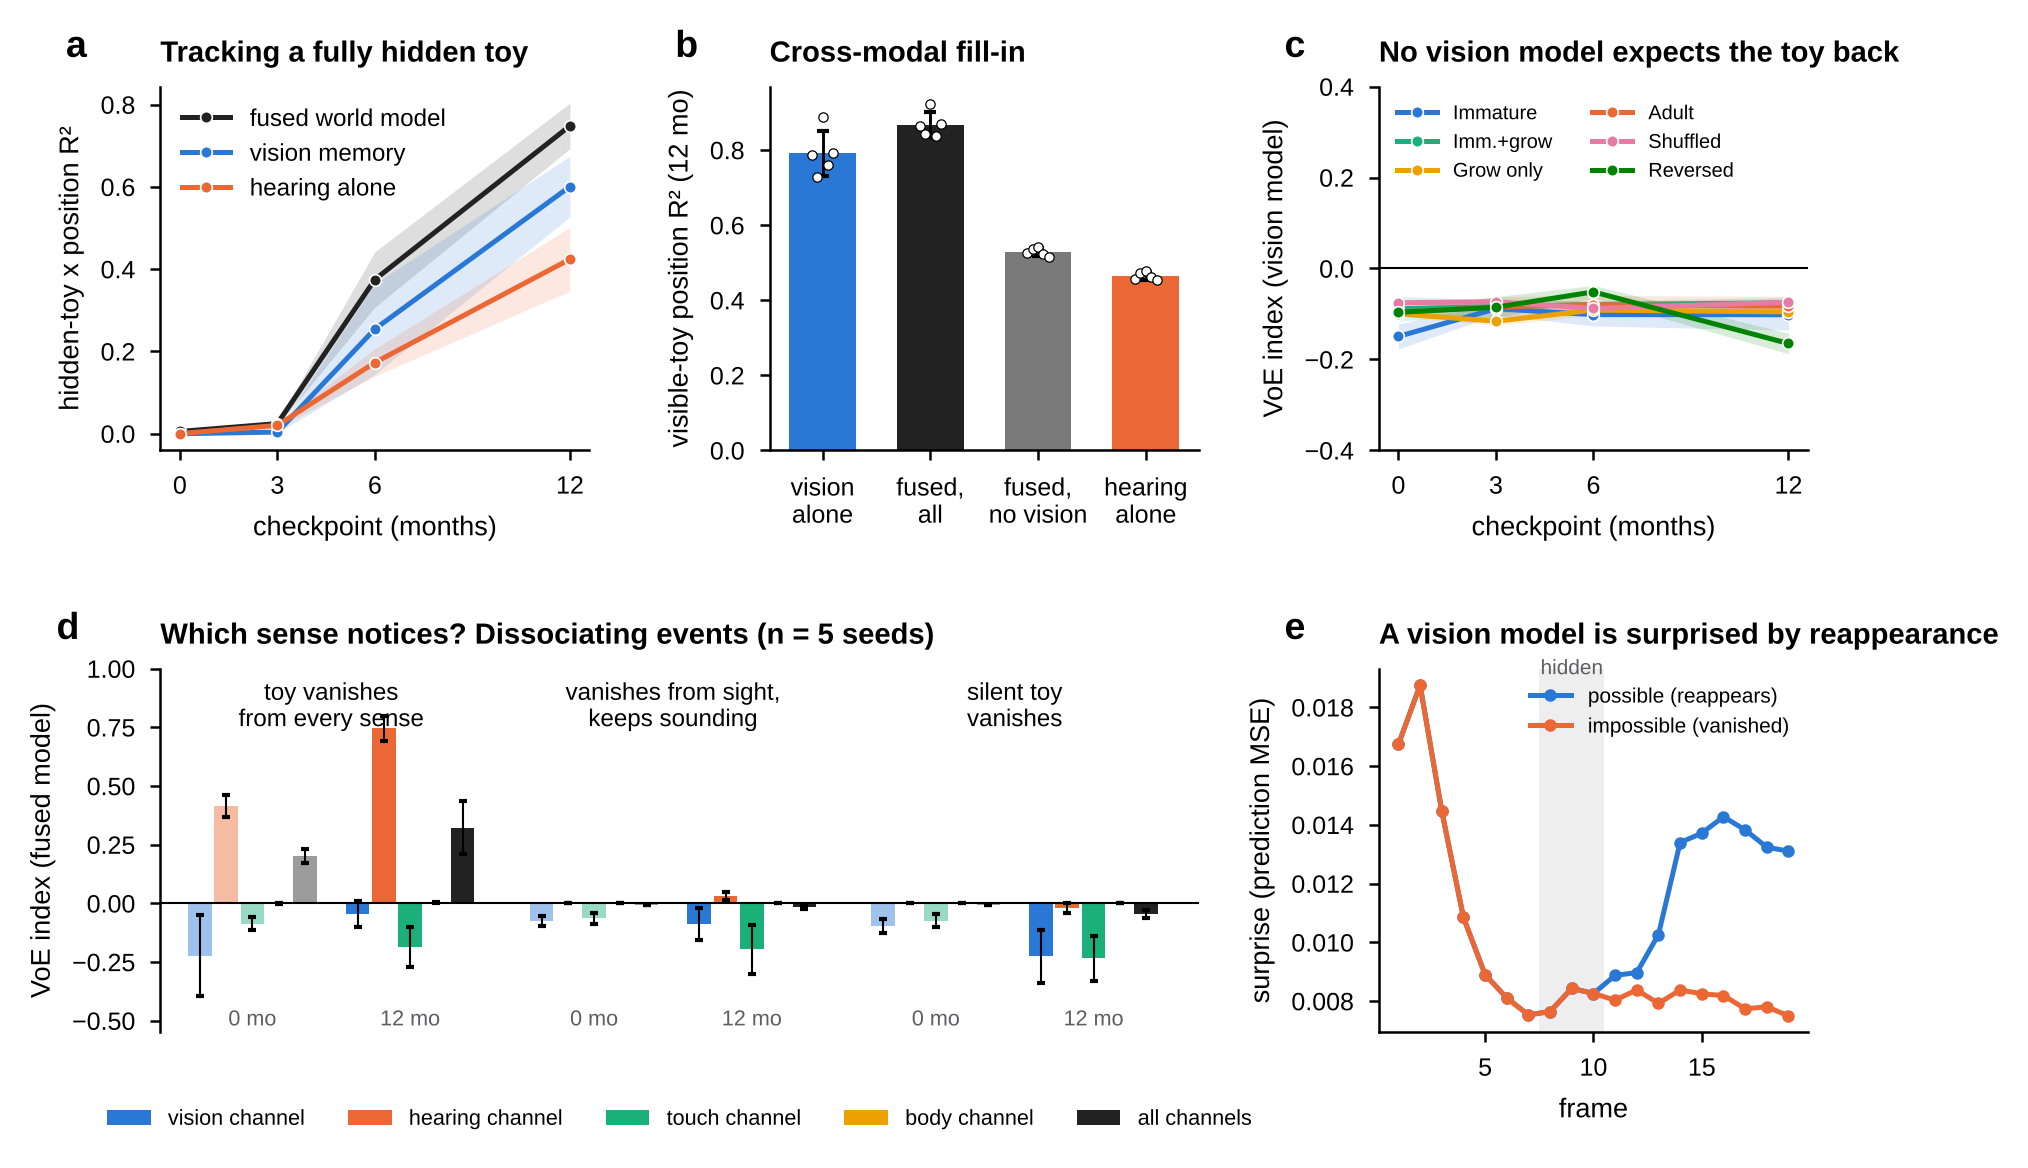
\includegraphics[width=1\textwidth,height=0.78\textheight,keepaspectratio]{fig4_fusion_expectation.png}
\caption{\textbf{Fusion and expectation.} \textbf{a}, Horizontal position of a fully hidden object decoded from the vision model's memory window, from audio alone and from the fused world model. \textbf{b}, Position of a visible object at the final checkpoint from vision alone, the fused state, the fused state with vision masked, and audio alone. \textbf{c}, Violation-of-expectation (VoE) index of the unimodal vision models; positive means more surprise when the object fails to reappear. \textbf{d}, VoE index of the fused model broken down by channel, for three events: the object vanishes from every modality; it vanishes from vision and touch but keeps sounding; a silent object vanishes. Faded bars, \(a=0\); solid, \(a=12\). \textbf{e}, Frame-by-frame surprise of one vision model (degraded-to-clean curriculum, final checkpoint) on a possible and an impossible event; grey, object hidden. Bands and whiskers, \ensuremath{\pm}1 s.d. over seeds.}
\label{fig:fusion}
\end{figure}

\textbf{No unimodal vision model is surprised by an object's disappearance.} No unimodal vision model, under any curriculum, has a positive violation-of-expectation index (Fig.~\ref{fig:fusion}c): all are more surprised when the object reappears than when it fails to, like a predictor that copies the last frame (Fig.~\ref{fig:fusion}e). This holds although the hidden object's position is decodable from the same model's memory. It is the behaviour Proposition~\ref{prop:surprise} predicts for a squared-error forecaster when the reappearance time is uncertain.

\textbf{The fused model is surprised only when a sound gives the event away.} The fused model does show a positive index when the object vanishes from every modality (0.32 \ensuremath{\pm} 0.11 at the final checkpoint), but its channels show where the surprise comes from: audio 0.75 \ensuremath{\pm} 0.05, vision \ensuremath{-}0.04 \ensuremath{\pm} 0.05 (Fig.~\ref{fig:fusion}d). The model registers that the sound stopped. When the object vanishes from vision but keeps sounding, the overall index is \ensuremath{-}0.02 \ensuremath{\pm} 0.01 and the vision channel \ensuremath{-}0.09 \ensuremath{\pm} 0.07; when a silent object vanishes, they are \ensuremath{-}0.04 \ensuremath{\pm} 0.02 and \ensuremath{-}0.23 \ensuremath{\pm} 0.11. Without a sound to give the event away, the fused model does not predict the object's return either: a read-out can show that information about a hidden object is present while the model's forecasts do not use it.

\textbf{Predicting an uncertainty, or predicting in latent space, does not produce surprise at disappearance.} Proposition~\ref{prop:surprise} attributes the missing surprise to a squared-error forecaster that predicts a conditional mean. We therefore tested two forecasters that predict something else (Appendix~\ref{app:followup}). A vision model whose forecast comes with a per-pixel variance, trained by the Gaussian likelihood, tracks the object as well as the main model (position \(R^2\) 0.85 \ensuremath{\pm} 0.04 at the final checkpoint) and still has a negative index in all five seeds (\ensuremath{-}0.35 \ensuremath{\pm} 0.23 by negative log-likelihood; \ensuremath{-}0.10 \ensuremath{\pm} 0.04 by squared error of the mean). A latent-space forecaster with a slowly updated target encoder and variance--covariance regularisation has a negative index in all five seeds as well (\ensuremath{-}0.22 \ensuremath{\pm} 0.14), but it does not learn to represent the object (position \(R^2\) 0.02 \ensuremath{\pm} 0.04), so this second test is uninformative about expectation (Extended Data Fig.~S4e, f). Predicting an uncertainty did not change the sign of the index, so the sign is not only a consequence of the squared-error loss; whether a latent objective that does track the object changes it remains open.

\textbf{Matching the amount of training to the stage leaves the final result unchanged.} In the staged curricula every stage receives the same number of updates. In a single run in which the operator's stage index rises linearly with the number of updates, so that the number of updates seen is proportional to \(a\), vision reaches position \(R^2\) 0.86 \ensuremath{\pm} 0.01 at \(a=12\), against 0.85 \ensuremath{\pm} 0.04 for the staged curriculum, and audio reaches 0.45 \ensuremath{\pm} 0.01 in both (Extended Data Fig.~S4a, b). The intermediate checkpoints differ, as they should: the matched vision model has had half as many updates at \(a=3\) as at \(a=6\), and reads out 0.03 \ensuremath{\pm} 0.02 and 0.67 \ensuremath{\pm} 0.05 there, against 0.29 \ensuremath{\pm} 0.16 and 0.74 \ensuremath{\pm} 0.06 in the staged curriculum. The final results do not depend on the choice of staging.

\section{Discussion}
\label{sec:discussion}

\textbf{What the theory explains.} Table~\ref{tab:predictions} sets each proposition against what we observed. The information bound and the learning-time law together account for the main shape of the vision learning curve under the degraded-to-clean curriculum: an operator that shrinks input variance and removes fine detail makes the early read-out both lower and slower, and the self-supervised model reaches only a small fraction of the ceiling until the operator sharpens. The growth delay accounts for why growing the network did not help, and the conditional-mean result accounts for the sign of the surprise index.

\begin{longtable}[]{@{}
  >{\raggedright\arraybackslash}p{(\columnwidth - 4\tabcolsep) * \real{0.3333}}
  >{\raggedright\arraybackslash}p{(\columnwidth - 4\tabcolsep) * \real{0.3333}}
  >{\raggedright\arraybackslash}p{(\columnwidth - 4\tabcolsep) * \real{0.3333}}@{}}
\caption{Predictions of the theory and what was observed.}\label{tab:predictions}\tabularnewline
\toprule\noalign{}
Proposition & Prediction & Observation \\
\midrule\noalign{}
\endfirsthead
\toprule\noalign{}
Proposition & Prediction & Observation \\
\midrule\noalign{}
\endhead
\bottomrule\noalign{}
\endlastfoot
1. Information bound & Learned score cannot exceed the ceiling at that input quality & Holds at every stage; early gap is large for vision \\
2. Learning time & Contrast scales speed by \(\kappa^{-2}\); blur limits the ceiling & Exact in the linear model; in the trained network, contrast-only reproduces the lag and blur-only barely slows learning \\
3. Growth delay & A plateau after each widening; fewer parameter-updates & Grown model lags; uses about half the parameter-updates \\
4. Conditional mean & Negative surprise index when reappearance is uncertain & Negative for every unimodal vision model; positive only when a sound gives the event away \\
\end{longtable}

\textbf{What it does not explain.} The propositions are exact for a linear read-out under gradient flow, whereas the networks we train are nonlinear and use Adam, so the theory and the experiments are linked by analogy and by ablation, not by derivation. The trained vision model lags its ceiling far more than the linear model lags its own, which suggests that most of the delay lies in learning features, not in fitting a read-out. Proposition~\ref{prop:time} does not apply as stated to adaptive optimisers, yet the ablations show that contrast, the component it singles out, still accounts for the early lag in the trained network. Extending the theory to deep linear networks \autocite{saxe2019mathematical} would close part of this gap and is future work. The Jacobian spectra of the trained encoders show the same ordering, coarse modes first, but we have not derived the delay for deep networks. Nor does the theory explain the benefit of degraded audio: the shuffled-order control points to augmentation, but we have not derived it.

\textbf{Implications for staged training.} Three design rules follow, each stated for the setting studied here. Reduce contrast or gain only if the cost in speed is acceptable, because with plain gradient descent it delays learning by the square of the scale and gives no lasting information benefit; use blur when the aim is to withhold fine detail early, and expect a lower ceiling in a finite budget; and do not use zero-initialised growth as a substitute for a schedule, because new units contribute nothing until their outgoing weights move. When surprise is the read-out, a squared-error pixel forecaster is a poor instrument in this setting. A forecaster that predicts a per-pixel variance and a latent-space forecaster were not surprised by the object's disappearance either, but the latent model did not learn to track the object at this scale \autocite{mohapatra2026senses}, so objectives that do, such as masked prediction over many patches and more data \autocite{garrido2025intuitive}, or training on longer horizons, remain to be tested against the same dissociating events.

\textbf{Limitations.} Everything is synthetic and small (\(32\times32\) scenes with one object, at most 0.6 million parameters per modality) and is evaluated mainly with linear probes, which measure decodability, not behaviour. We did not test whether these curricula help or hurt larger architectures or standard benchmarks, so the findings describe this setting and are not evidence about training at scale. Maturity is defined by the task: touch reaches its final level at once because tracking the object needs no fine tactile discrimination, and a harder tactile task would give a different order. The theory is exact for a linear read-out under gradient flow and is suggestive for trained networks. The audio, tactile and proprioceptive operator tables are placeholders, and the stage labels carry no claim about hours of experience. With 5 seeds per curriculum, several comparisons have large effect sizes but are not significant (Fig.~\ref{fig:costs}c); we report them as estimates. The Jacobian spectra describe the encoder and not the map to the read-out, and the experience-matched curriculum has no \(a=0\) checkpoint (its first is at \(a=1\)).

\textbf{Future work.} The immediate extensions are late fusion with modality onset order as a factor; comparing the biological order of modalities (touch, then audio, then vision) with artificial and arbitrary orders for multisensory integration; latent-space objectives, with an inductive bias or masking strategy that lets them survive strong blur, tested against the dissociating events; and extending the theory to deep linear networks and measuring the delay from the Jacobian spectrum. The decisive tests are at scale: whether staged input improves sample efficiency or robustness on standard benchmarks and with modern architectures, in a 3D embodied environment and on real egocentric video. The data path runs from this synthetic environment to an embodied simulator for touch and proprioception \autocite{mattern2024mimo} and to head-camera corpora for vision and audio \autocite{sullivan2021saycam,long2024babyview}.

\clearpage
During the preparation of this work, the author used an AI assistant (Claude, Anthropic) to help write and run analysis code, draw figures and draft text. The author reviewed and edited the content and takes full responsibility for the content of the publication.

All code, configurations, results and trained checkpoints are at \url{https://github.com/pikulsomesh/developmental-world-models} (MIT licence). The data are synthetic and are regenerated by the code from the random seeds listed in the repository.

S. Mohapatra conceived the study, directed the work and approved the final text.

This work received no specific funding and was carried out independently.

The author declares that there is no conflict of interest regarding the publication of this article.

\printbibliography

\clearpage
\appendix
\section{Experimental details}
\label{app:details}

\subsection{Environment}
\label{app:env}

Episodes last 20 frames. An object of type \(c\in\{1,\dots,4\}\) moves with constant velocity and bounces in a \(32\times32\) scene; the effector's position follows a smoothed random action \(u_t\in\mathbb R^2\) and stays in the lower half. Half the episodes contain a vertical screen. Vision is an RGB image on a dark background; the object is drawn with a type-specific shape and colour, the screen in grey and the effector in a fixed colour. Audio is a binaural spectrum, \(o^{\text{aud}}_t\in\mathbb R^{2\times32}\), a Gaussian bump at a type-specific pitch whose loudness falls with distance and whose left/right balance follows horizontal position; sound passes through the screen. Touch is an \(8\times8\) image of the object's shape when the effector overlaps it, otherwise zero. Proprioception is the effector's normalised position and velocity. Ground truth includes object position, type, visibility and contact. Training sets have 3,000 episodes per seed and test sets 400.

\textbf{Probe events.} \emph{Possible}: the object crosses a central screen horizontally and reappears. \emph{Impossible}: the object vanishes while hidden, from every modality. \emph{Vanish-visual}: it vanishes from vision and touch but keeps sounding as if still moving. \emph{Silent}: possible and impossible events with no sound (audio receives noise only). \emph{Track}: like possible, with a wider screen (14 px) and varied speed, so the object is hidden for about seven frames. Paired events share random draws so that they differ only in the manipulation.

\subsection{Non-visual degradation operators}
\label{app:frontends}

\emph{Audio.} Per channel, \(x=g_{\beta(a)}*o\) along frequency, then a high-frequency roll-off \(x_f\leftarrow x_f\,\mathrm{sigmoid}\big((h(a)\cdot32-f)/1.5\big)\), then reduced interaural difference \(x_{L,R}\leftarrow m+\rho(a)(x_{L,R}-m)\) with \(m=\tfrac12(x_L+x_R)\), then additive Gaussian noise \(\eta(a)\). \emph{Touch} and \emph{proprioception.} Receptive-field blur \(G_{\tau(a)}\) on the \(8\times8\) patch plus noise; additive noise on proprioception.

\subsection{Training}

Adam \autocite{kingma2015adam}, learning rate \(2\times10^{-3}\), batch 32, 2,000 updates per stage for vision and 1,500 for the other modalities, four stages in one continuous run; weights carry over between stages and a fresh Adam optimiser is started at each stage, so all curricula see the same optimiser schedule. Hyperparameters were set once on the degraded-to-clean curriculum and shared by all curricula. Seeds: 5 for each curriculum (fusion uses the grown curriculum's checkpoints). Growing vision models go from 43,507 to 586,499 parameters and growing audio models from 13,792 to 149,088. Training compute is approximated by \(\sum_{\text{stages}}(\text{parameters})\times(\text{updates})\); relative to a fixed network of the largest size, grown vision models use 0.48 and grown audio models 0.49. The fusion model uses projections to 64 dimensions, latents standardised per modality, and a modality masking probability of 0.3.

\subsection{Spectral analysis}

For each stage we generated 800 episodes without occluders, kept the 6,000 frames in which the object is visible, applied the vision operator, centred the pixels and computed the covariance \(\Sigma\) (\(3{,}072\times3{,}072\)) and its cross-covariance with the standardised object position. The closed-form solution of Proposition~\ref{prop:time} gives \(R^2(t)\), the linear ceiling \(\sum_i c_i^2/\lambda_i\) (modes with \(\lambda_i<10^{-9}\lambda_{\max}\) are dropped, which acts as a numerical noise floor) and the time to half the ceiling, found by bisection. The step size is fixed at \(1/\lambda_{\max}\) of the clean input so that every stage is stable under the same step. We verified the closed form against explicit gradient descent at \(a=0\) (agreement to \(10^{-3}\) in \(R^2\)). Controlled sweeps scale contrast or blur alone, with the operator otherwise clean.

\subsection{Read-outs}

\textbf{Linear probes.} For features \(X\) (a latent, or a memory window of latents) and targets \(Y\) we use ridge regression with centred targets and an unpenalised intercept,
\begin{equation}\hat B=\arg\min_B\lVert (Y-\bar Y)-X_cB\rVert^2+\lambda\lVert B\rVert^2=(X_c^\top X_c+\lambda I)^{-1}X_c^\top(Y-\bar Y),\end{equation}
where \(X_c\) are the standardised features, and score \(R^2=1-\sum\lVert y-\hat y\rVert^2/\sum\lVert y-\bar y\rVert^2\) on test episodes. Touch is probed on contact frames and proprioception on effector position.

\textbf{Information ceiling.} For every modality and each stage \(a\in\{0,1,2,3,4,6,9,12\}\) the supervised network is trained for 1,500 updates on single filtered frames and scored on held-out frames.

\textbf{Violation of expectation.} With \(S_{\text{pos}}\) and \(S_{\text{imp}}\) the mean surprise on paired possible and impossible events, the effect size is \(d_z=\overline{S_{\text{imp}}-S_{\text{pos}}}/\mathrm{sd}(S_{\text{imp}}-S_{\text{pos}})\).

\textbf{Occluded tracking.} Probes are fitted on half of the \emph{track} episodes and tested on the other half.

\subsection{Follow-up experiments}
\label{app:followup}

All follow-up experiments use the main study's full-size networks, data generator, optimiser and seeds (0--4), and report the own-stage probe.

\textbf{Experience-matched curriculum.} One network is trained in a single run of four times the per-stage number of updates, in which the stage index rises linearly with the update count from 0 to 12; checkpoints are taken after 1/12, 3/12, 6/12 and 12/12 of the updates.

\textbf{Uncertainty-aware forecaster.} The vision model gains a second decoder with the same architecture whose sigmoid output is scaled to a log-variance \(\log\sigma^2_q\) between \(-7\) and \(1\) for every pixel \(q\) of the forecast. It is trained on the Gaussian negative log-likelihood \(\tfrac12\big(\log\sigma^2_q+(\tilde o_{t+1,q}-\hat o_{t+1,q})^2/\sigma^2_q\big)\) with the same motion weights, on detached inputs (the predicted latent and the predicted mean), so the forecaster itself receives exactly the main-study gradients and the head learns how uncertain that forecaster is. Surprise is the unweighted mean of the negative log-likelihood over pixels; the squared error of the mean is also reported.

\textbf{Latent forecaster.} The decoder is removed and the dynamics module predicts the next frame's code from a target encoder whose weights are an exponential moving average (rate 0.99) of the encoder's, with no gradient through the target, plus variance and covariance penalties on the codes (weights 25, 25 and 1). Surprise is the mean squared error between the predicted code and the target encoder's code of the next frame. This is the model trained in the companion paper, and the same runs are used.

\textbf{Index for these forecasters.} The index uses the same events and frames as the main study, \((S_{\text{imp}}-S_{\text{pos}})/(|S_{\text{imp}}|+|S_{\text{pos}}|)\); the absolute values leave it unchanged when the surprises are positive and keep it bounded when a negative log-likelihood is negative.

\textbf{Jacobian spectrum.} For each vision checkpoint of the degraded-to-clean and clean curricula (seeds 0--4; seed 0 from the stored checkpoints, seeds 1--4 retrained with identical settings and reproducing the main-study read-outs exactly) we took 400 clean frames in which the object is visible, computed the Jacobian of the 32-dimensional latent with respect to the 3,072 input values for each frame by automatic differentiation, and expressed it in the principal directions of the clean frames. The energy of mode \(k\) is \(\sum_n\lVert J_nv_k\rVert^2\); the share in the top 10 and 100 modes and the effective rank \((\sum_i\sigma_i)^2/\sum_i\sigma_i^2\) of the frame-averaged Jacobian are reported.

\subsection{Statistics}

Bands and whiskers are \ensuremath{\pm}1 s.d. over seeds. Planned comparisons at the final checkpoint use Welch's t-test and Hedges' \(g=\frac{\bar a-\bar b}{s_p}\big(1-\frac{3}{4(n_a+n_b)-9}\big)\), where \(s_p\) is the pooled standard deviation of the two groups, with approximate 95\% interval \(g\pm1.96\sqrt{\frac{n_a+n_b}{n_an_b}+\frac{g^2}{2(n_a+n_b)}}\). No correction for multiple comparisons is applied; Table~\ref{tab:stats} lists all planned comparisons.

\begin{longtable}[]{@{}llll@{}}
\caption{Planned comparisons.}\label{tab:stats}\tabularnewline
\toprule\noalign{}
Comparison (final checkpoint) & Hedges' g & p (Welch) & n \\
\midrule\noalign{}
\endfirsthead
\toprule\noalign{}
Comparison (final checkpoint) & Hedges' g & p (Welch) & n \\
\midrule\noalign{}
\endhead
\bottomrule\noalign{}
\endlastfoot
Vision clean, degraded-to-clean vs clean baseline & \ensuremath{-}1.2 & 0.06 & 5/5 \\
Vision clean, grown vs fixed (degraded-to-clean) & \ensuremath{-}1.0 & 0.11 & 5/5 \\
Vision identity, grown vs fixed (degraded-to-clean) & \ensuremath{-}2.2 & 0.005 & 5/5 \\
Vision on \(a=0\) input, degraded-to-clean vs clean baseline & 0.9 & 0.16 & 5/5 \\
Audio clean, degraded-to-clean vs clean baseline & 1.5 & 0.05 & 5/5 \\
Audio clean, grown vs growth only & 1.6 & 0.05 & 5/5 \\
Hidden object, fused vs vision memory & 1.8 & 0.01 & 5/5 \\
\end{longtable}

\subsection{Order of maturation under the information ceiling}
\label{app:milestones}

For each modality, the half-ceiling stage is the first stage at which the information ceiling reaches half of its final value (position \(R^2\) for vision and audio; identity accuracy above chance for touch). It is touch 0, audio 4 and vision 0, so Kendall's \ensuremath{\tau} against the order of functional maturity usually described for biological learners, touch before audio before vision \autocite{turkewitz1982limitations}, is 0.00 (Fig.~\ref{fig:development}f): the ceiling-based measure does not recover that order, because the stage-0 vision input still supports coarse localisation even though the learned model does not.

The study uses only synthetic data; no human or animal participants were involved.

\clearpage
\section*{Extended Data (Supplementary Figures)}
\setcounter{figure}{0}
\renewcommand{\thefigure}{S\arabic{figure}}

\begin{figure}[htbp]
\centering
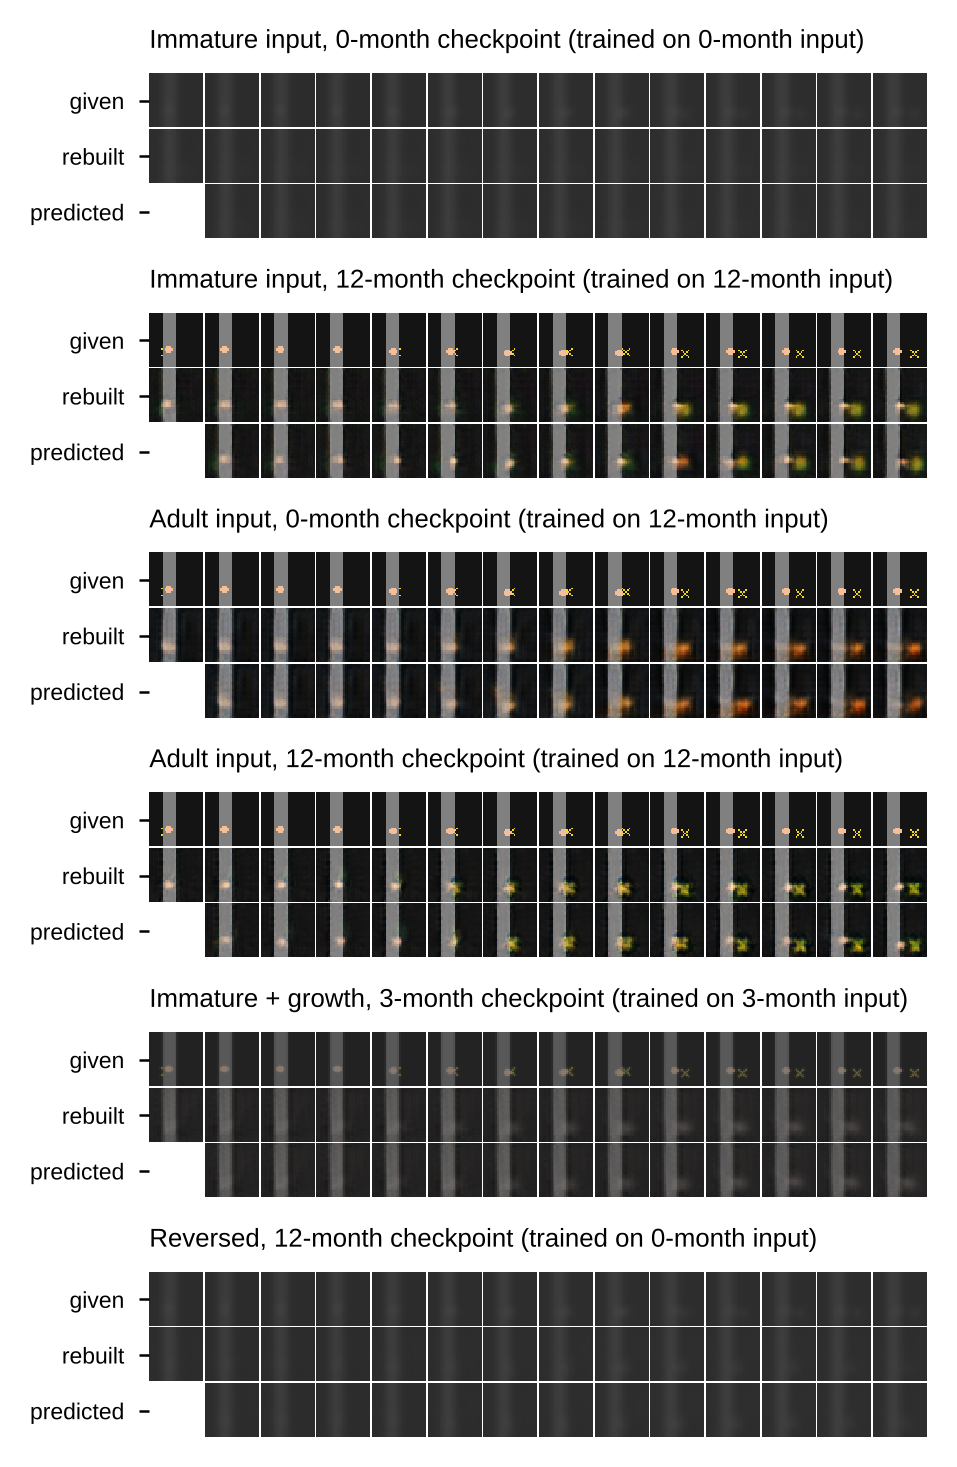
\includegraphics[width=1\textwidth,height=0.78\textheight,keepaspectratio]{ed1_model_outputs.png}
\caption{\textbf{What the vision models see, reconstruct and predict.} For selected curricula and checkpoints: the input given (at the stage that checkpoint was trained on), the reconstruction from the latent, and the one-step prediction, for the first 14 frames of one episode.}
\end{figure}

\begin{figure}[htbp]
\centering
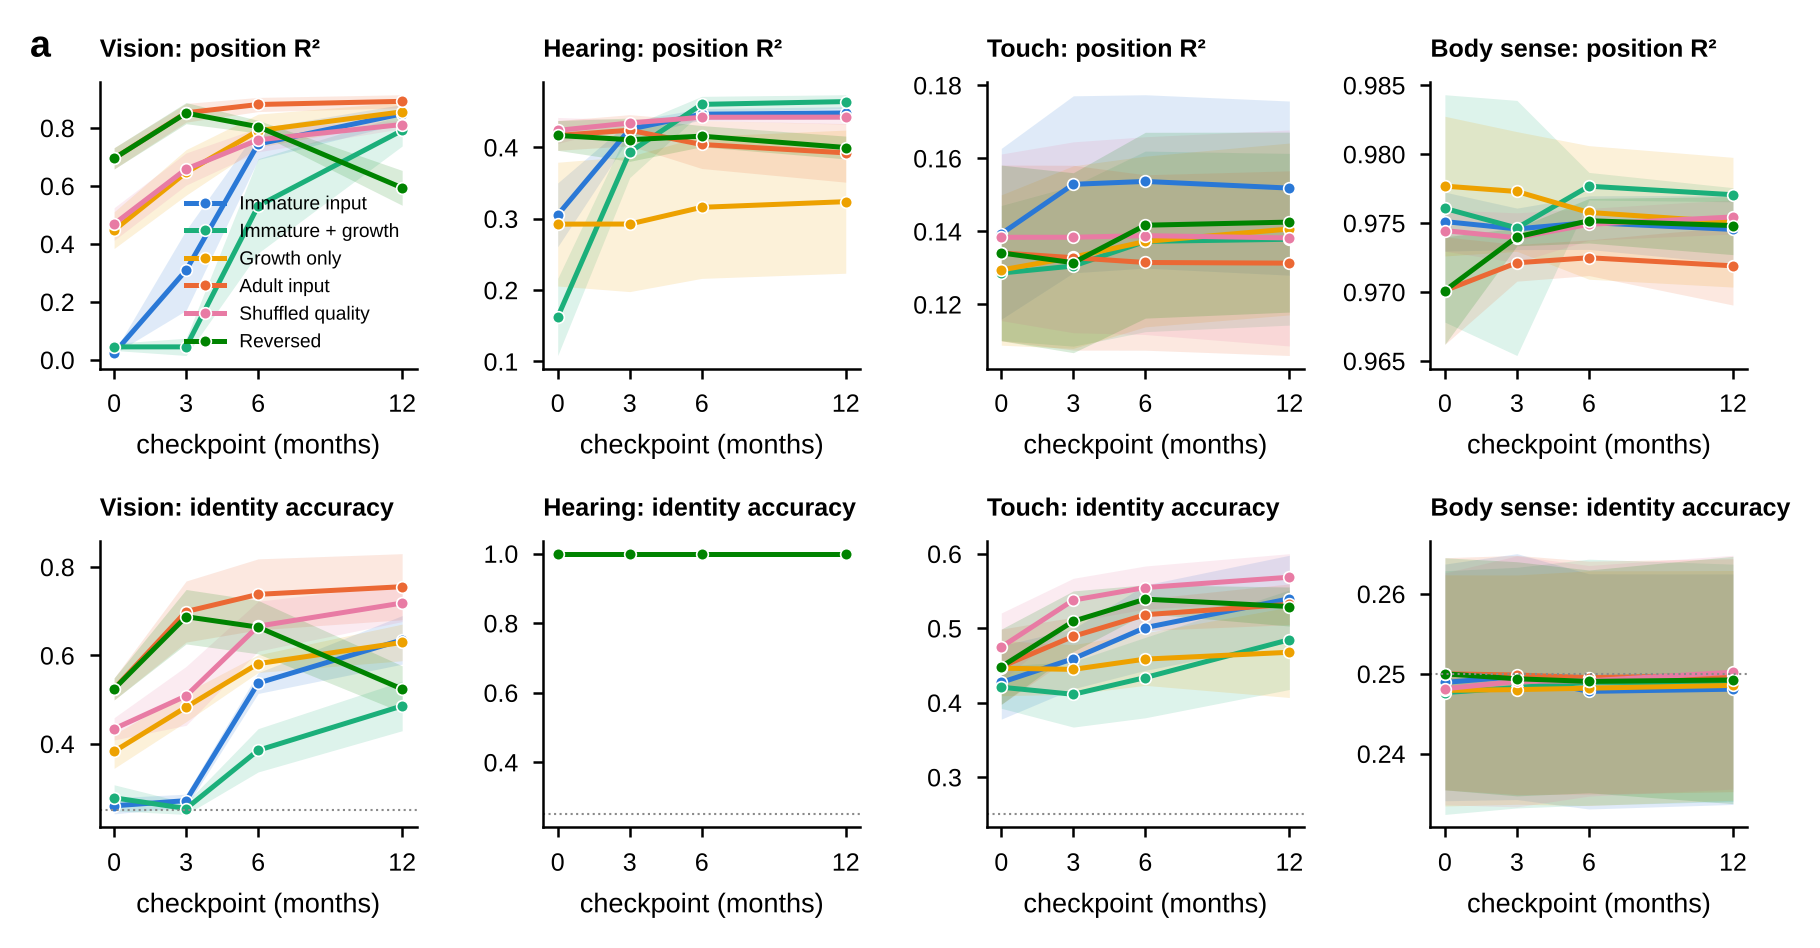
\includegraphics[width=1\textwidth,height=0.78\textheight,keepaspectratio]{ed2_all_senses.png}
\caption{\textbf{All modalities, all curricula.} Position \(R^2\) (top) and identity accuracy (bottom; dotted, chance) per checkpoint.}
\end{figure}

\begin{figure}[htbp]
\centering
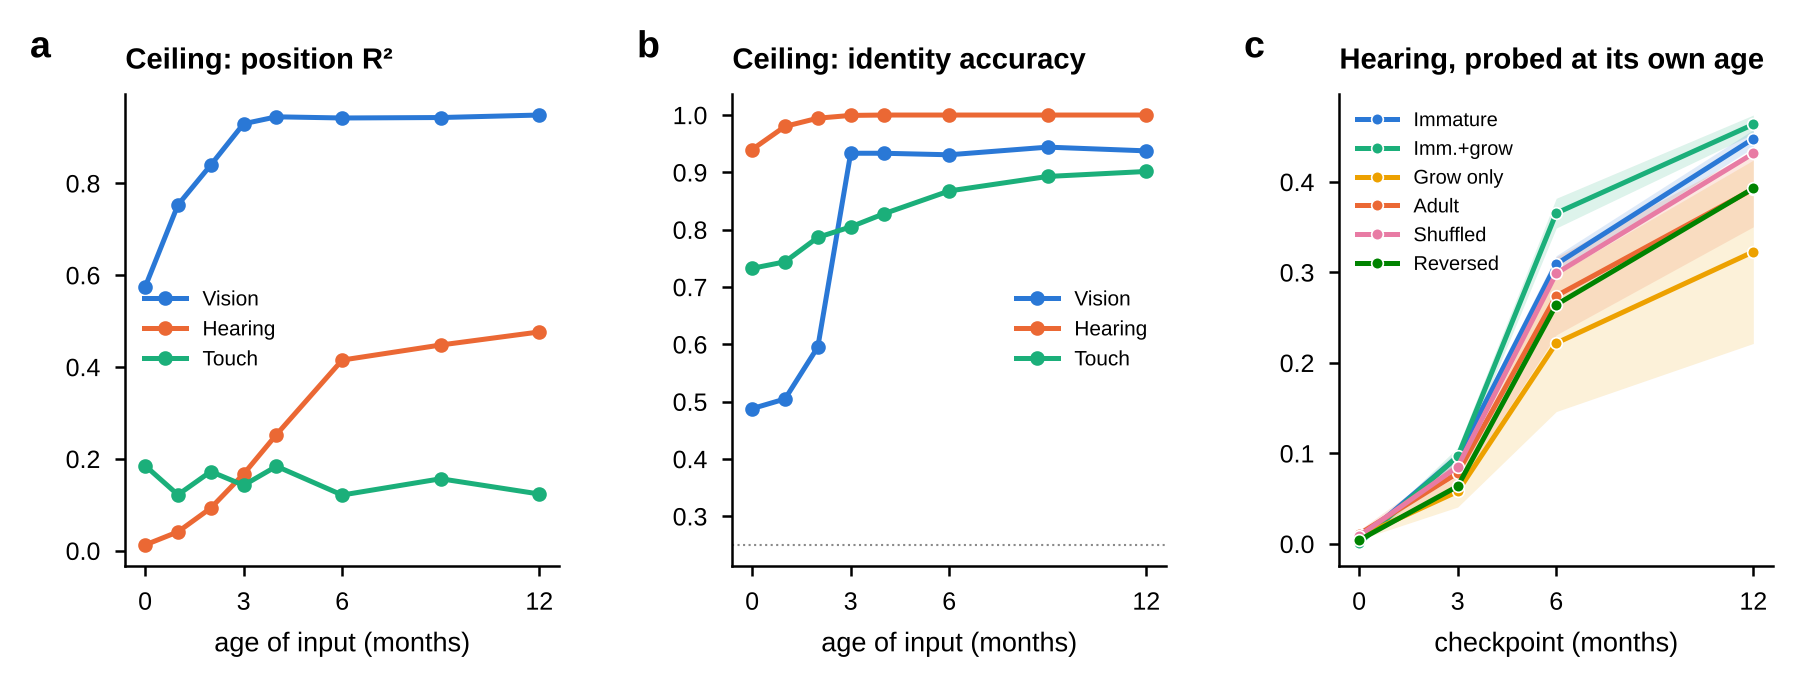
\includegraphics[width=1\textwidth,height=0.78\textheight,keepaspectratio]{ed3_ceiling_ownage.png}
\caption{\textbf{Information ceilings and own-stage probes.} The same ceiling data are plotted by stage in the companion paper \autocite{mohapatra2026senses}. \textbf{a}, \textbf{b}, Supervised ceilings per modality and stage. \textbf{c}, Audio probed on own-stage input.}
\end{figure}

\begin{figure}[htbp]
\centering
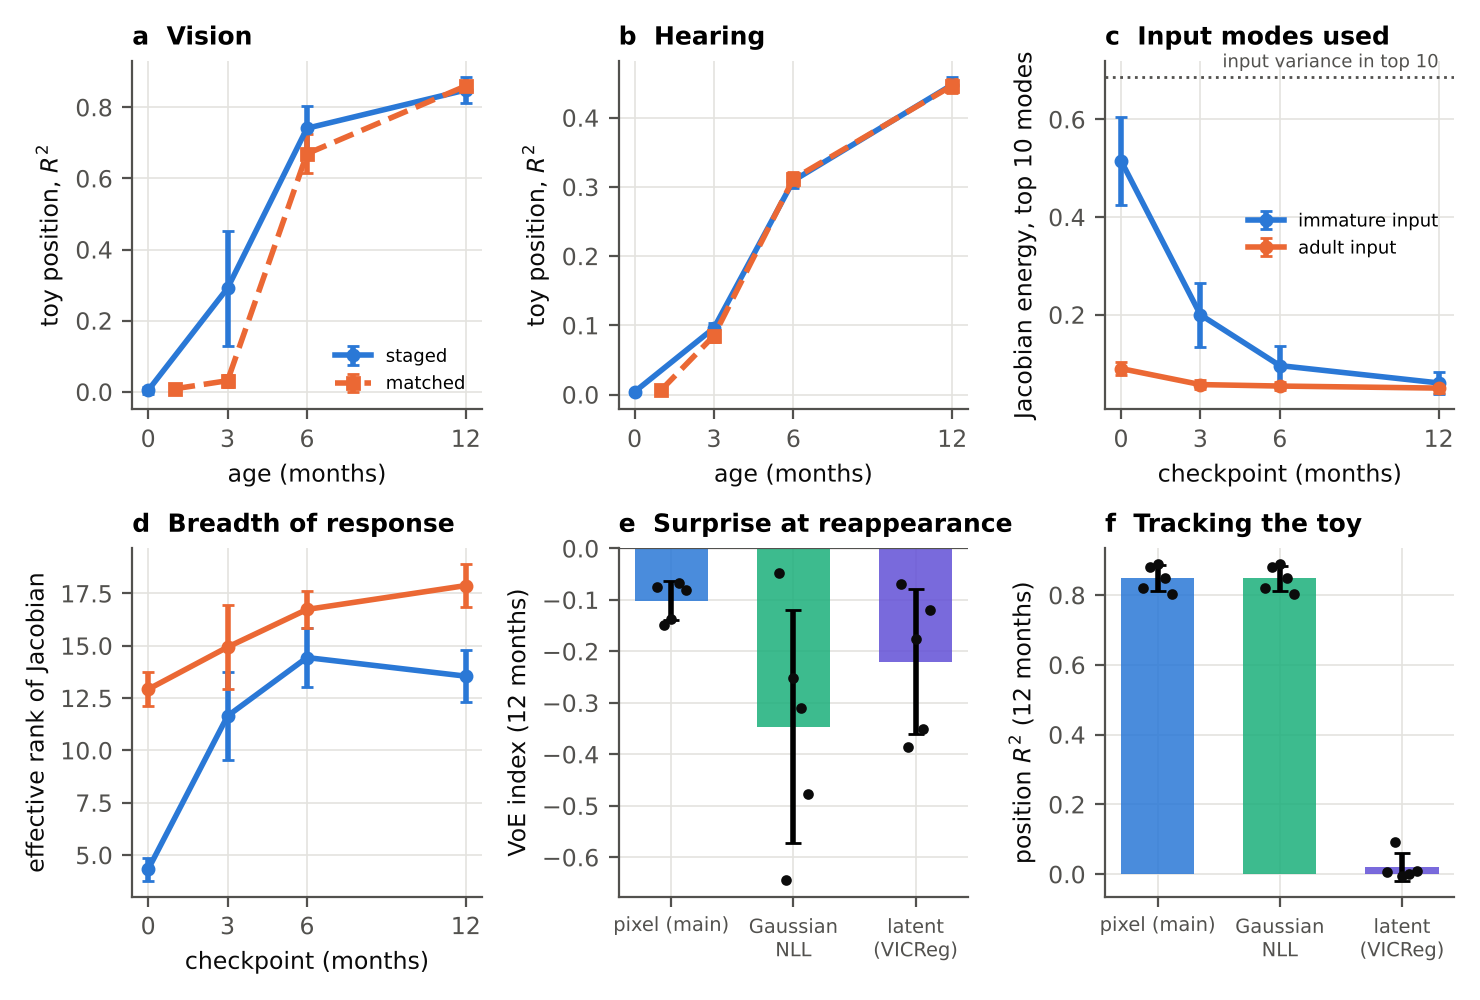
\includegraphics[width=1\textwidth,height=0.78\textheight,keepaspectratio]{ed4_future_work.png}
\caption{\textbf{Follow-up experiments.} \textbf{a}, \textbf{b}, Object position read-out for vision (\textbf{a}) and audio (\textbf{b}) in the staged curriculum (equal updates per stage) and in a single run in which the number of updates is proportional to the stage index (matched; first checkpoint at \(a=1\)). \textbf{c}, \textbf{d}, Jacobian of the vision encoder on clean frames, in the principal directions of the clean input: share of its energy in the ten leading modes (\textbf{c}; dotted line, share of the input variance in those modes) and effective rank (\textbf{d}), for the degraded-to-clean and clean curricula. \textbf{e}, Violation-of-expectation index at the final checkpoint for the main pixel forecaster, a forecaster with a predicted variance (negative log-likelihood) and a latent-space forecaster. \textbf{f}, Position \(R^2\) of the same three models. Lines and bars, mean over 5 seeds; whiskers, \ensuremath{\pm}1 s.d.; dots, seeds.}
\end{figure}

\end{document}
